\chapter{Introduction}
\label{chap:intro}

%This is the first Chapter.  Here is an example citation:
%\citet{rountree98}.

%%%%%%%%%%%%%%%%%%%%%%%%%%
%% meta-text / overview %%
%%%%%%%%%%%%%%%%%%%%%%%%%%

The thesis presents research into genetic interactions based on \gls{genomics} data and \gls{bioinformatics} approaches. This Chapter introduces the recent developments in \gls{genomics} and \gls{bioinformatics}, particularly in their application to cancer research. \Gls{synthetic lethal} interactions are a long standing area of research in genetics in both model organisms and cancer biology. Various reasons why these interactions are of interest in fundamental and translational biology will be outlined but first these and similar interactions will be defined. A \gls{bioinformatics} approach to \gls{synthetic lethal} interactions enables much wider exploration of the inter-connected nature of genes and proteins within a cancer cell than previous candidate-based approaches. An alternative approach is experimental screening which will be presented and contrasted with \gls{bioinformatics} approaches in more detail.  An emerging application of \glspl{synthetic lethal} is the design of treatments with specificity against loss of function mutations in tumour suppressor genes. \gls{E-cadherin} (encoded by \textit{CDH1}) is a prime example of this which will be the focus of the analysis in this thesis and as such the role of this gene in cellular and cancer biology will be briefly reviewed.   


%%%%%%%%%%%%%%%%%%%%%%%%%%%%%%%%%%%%%%%%%%%%%%%%%%%%%%%%%%%%%%%%%%%%%%%%%%%
%%%%%%%%%%%%%%%%%%%%%%%%%%%%%%%%%%%%%%%%%%%%%%%%%%%%%%%%%%%%%%%%%%%%%%%%%%%

\section{Cancer Research in the Post-Genomic Era}

\Gls{genomics} technologies have the potential to vastly impact upon various areas including health and cancer medicine. Considering the progress in recent \gls{genomics} research, this technology and the findings from it have considerable potential for significant impacts in the clinic and wider applications of genetics either directly or by enabling more focused genetics research on candidates selected from \gls{genomics} or \gls{bioinformatics} analysis. The completion of the draft Human Genome \citep{Lander2001} marks a major accomplishment in genetics research and raises new challenges to utilise this genomic scale information effectively. Technologies in this area have rapidly developed since completion of the human genome project and many global large-scale projects have expanded upon the human genome, to populations \citep{1000Genomes2010}, to cancers \citep{Dickson1999, ICGC2011}, and to deeper functional understanding \citep{ENCODE2004, FANTOM2001}. However, impact on the clinic has been slower than initially anticipated following the completion of the ``draft'' genome with \gls{genomics} technologies yet to become widely adopted in healthcare and oncology. Here we outline the \gls{genomics} technologies and \gls{bioinformatics} approaches which have led to availability of \gls{genomics} data and techiques used in this thesis and potential for applications in cancer research or the clinic in the future. 

\subsection{Cancer as a Global Health Concern}

Cancer is a class of diseases involving malignant cellular growth, invasion of tissues, and spread to other organs. While there are also environmental factors, most cancers occur more frequently with age and family history. Accordingly, genetics has become widely acknowledged as having an important role in cancer risk (in addition to environmental factors). Cancers arise from dysregulated cellular growth or differentiation from stem cells. These can occur through genetic mutations or alterations in gene regulation or expression.

Cancers are a major global health concern, being the second leading cause of death globally \citep{WorldHealthOrg2017}, with an estimated annual incidence of 14.1 million cases and annual mortality of 8.2 million people \citep{Ferlay2015}. Breast and stomach cancers are among the 5 most frequent cancers globally, with breast cancer affecting women more than other cancer tissue types. Breast cancer has an estimated annual incidence of 1.6 million cases and mortality of 520 thousand people. Stomach cancer has an estimated annual incidence of 950 thousand cases and a mortality of 723 thousand people. Cancer is also a major health concern here in New Zealand, with 19.1 thousand people (including 2.5 thousand cases of breast cancer and 370 cases of stomach cancer) diagnosed annually \citep{CIX2013}, among the highest incidence (age-standardised per capita) of cancer in the world \citep{Ferlay2015}.   

While the genetic contribution to cancer risk and many of the molecular changes occurring in cancers are widely acknowledged \citep{CancerResearchUK2017, ASCO2017, CSNZ2017}, the majority of these findings have yet to impact on clinical practice. Diagnostics are traditionally based on pathological examination of tissue samples where histological staining for cell type, biomolecules and biomarkers continue to be widely used, although genetic and biochemical markers are being adopted for some cancer types. In general, the current standard of care includes surgery, radiation, and cytotoxic chemotherapy, depending on whether the cancer is localised or has become systemic (via metastasis) and spread to other organ systems. These approaches can be effective against certain cancers, particularly in early stage cancer or in patients with particular subtypes (such as acute myeloid leukaemia) which respond well to modern treatment regimens. Thus early diagnosis is important to patient survival and quality of life. National screening programs (which prioritise patients with a high risk of cancer) therefore aim to diagnose cancers early and subtypes more accurately. Therefore identification of patients with genetic variants or family histories (for inclusion in national databases) for high risk of particular cancers is an important health issue, particularly where effective interventions exist if these cancers are diagnosed early. Thus high risk individuals being regularly monitored for some cancers are sometimes offered preventative surgery or treatment for pre-cancerous tissue \citep{Guilford2010, Scheuer2002}. 

Chemotherapy is a last-resort treatment for many advanced stage (systemic) cancers which is designed to inhibit the growth and spread of cancer throughout the body by targeting rapidly growing cells. However, this approach often has severe adverse effects, a narrow therapeutic window, and is not suitable for chemopreventative application in many cases \citep{Kaelin2009}. Since surveillence preventative surgery (removing the tissue at risk of cancer) is not completely effective at preventing cancers and may impact on quality of life, depending on the cancer tissue types they are at risk of, alternative treatment strategies based on molecular biology and other fields are being investigated. These alternatives include immunological, endocrine, and targeted therapeutics, with a particular interest in treatments with specificity against cancer cells and wider applications (i.e., tolerable effective doses in applciations as a chemopreventative or against advanced stage cancers).

%Fran: clinical assistance (Sharon Pattison).
%% after Parry/Aug/Anita?


\subsubsection{The Genetics and Molecular Biology of Cancers}

Cancers involve dysregulation of genes with both somatic mutations or regulatory disruptions which accumulate during a patient's lifetime and germline mutations which predispose individuals to high-risk early onset cancers \citep{NCI2015, ACS2017, Guilford1998}. Cancer is widely viewed to be a genetic disease due to these familial cancer syndromes, hereditary risk factors, and the molecular changes occurring in cancers, including numerous cancer genes which have been identified \citet{Stratton2009, Vogelstein2013}. Cancer genes are generally classified into two classes: ``oncogenes'' which are activated in cancers, driving tumour growth and invasion, or ``tumour suppressors'' which are inactivated in cancers, removing cellular regulation and genomic maintenance functions. The mutations which cause cancers accumulate with age and have been suggested to be inevitably coupled with aging due to the association of cancer incidence with the stem cell divisions in which mutations could occur across tissue types \citep{Tomasetti2015}.  

%Cancer is Genetic:
%National Cancer Institute \citep{NCI2015} Hereditary Cancer syndromes, somatic mutations, genetic testing / seq
%American Cancer Society \citep{ACS2017} genes in cancer, familial snydromes, testing
%Cancer Research UK \citep{CancerResearchUK2017} genes and family history
%American Society of clincal oncology (cancer.net) \citep{ASCO2017} somatic and germline mutations
%Cancer Society of NZ \citep{CSNZ2017} loss of control, e.g., mutation, screening, improved detection

%\subsubsubsection{Hallmarks of Cancers}
\citet{Hanahan2000} identified several key molecular and cellular traits shared across most cancers as a rational approach to the complex changes that occur in cancer initiation and progression due to common molecular machinery underlying all cells. A cancer cell must possess limitless replication potential, modulate growth signals to grow indefinitely, and gain invasive or metastatic capabilities. In addition, cancers must evade apoptosis, the immune system, and sustain angiogenesis and energy metabolism in order to survive \citep{Hanahan2011, Hanahan2000}. In order to achieve this, cancer cells undergo changes to their genomes and the surrounding cells to create a tumour microenvironment. Thus genomic instability has a key role in the survival and proliferation of cancer cells and the progression of further disease, as these malignant characteristics are acquired. Identifying the mechanisms of these acquired traits and the underlying genetic mutation or dysregulation behind them, such as \gls{E-cadherin} mutation in metastasis or p53 mutation in genomic instability \citep{Hanahan2000}, will be an important step in understanding and inhibiting cancer with the next generation of genomically-informed treatments. 

Molecular biological processes have particular importance in characterising breast cancers. Gene expression and regulatory signals confer cell identity and response to the environment. Therefore gene expression has been investigated with microarray technologies \citet{Perou2000}, with ``intrinsic subtypes'' identified characterised by estrogen receptor, \textit{HER2}, and basal, epithelial signalling. The expression profiles were similar across independent samples of the same tumour and  between primary and metastatic tumours of the same patient. Thus expression profiles represent the molecular state of a tumour rather than the sample and the molecular configuration of the cells regulation is carried through the cellular lineage of during metastasis preserving the molecular subtype. These molecular intrinsic subtypes ``luminal A'', ``luminal B'', ``HER2-enriched'', ``basal-like'', and ``normal-like'' have been replicated across microarray studies \citep{Hu2006}, with their relevance to prognosis (including predicting survival and response to neoadjuvant chemotherapy) demonstrated and a 50-gene subtype predictor from microarray and \gls{qPCR} analysis has been provided \citep{Sorlie2001, Parker2009}. This has been further updated with the ``claudin-low'' subtype \citep{Herschkowitz2007} and stimulated further investigations into subtyping of breast cancers by molecular properties.

Despite differences in subtyping performed by different research groups and companies, there is widespread agreement that distinguishing luminal, HER2-enriched, and triple negative tumours can be performed with expression profiles and have value in our understanding of cancer progression and prognostic importance for patients \citet{Dai2015}. High-throughput technologies have the potential to enable such subtyping on a vast scale in discovery of further subtypes in breast cancer or other diseases and in identification of these subtypes along with mutations in routine clinical diagnostic and prognostic testing. The ``Pan cancer'' approaches by the cancer genome atlas project (as discussed in more detail in Section~\ref{TCGA_Findings}) expand on the importance of molecular differences between cancers by examining molecular profiles across cancer tissue types \citep{TCGA2013PAN}.

The molecular variability of cancer has also been approached rationally at a pathway level with patients subgroups activating different molecular pathways reflecting differences in disease mechanisms \citep{Gatza2010}. A robust approach to measuring pathway activation in cancer is with a``metagene'' which gives a consistent signal as a consensus of expression across genes even if they are inversely correlated \citep{Huang2003, Anjomshoaa2008, Nagalla2013}. These are derived from the first principal component or eigenvector of a singular matrix decomposition, capturing the the most consistent variation across genes in a pathway or gene signature. \citet{Gatza2010} used gene signatures for 18 cellular pathways in breast cancer to define subtypes with distinct molecular pathway activity. In a meta-analysis of Affymetrix microarray expression data for 1,143 samples and 50 cell lines, unsupervised hierarchical clustering robustly defined subtypes with common homogeneous pathway activity despite variation in the specific mutations giving rise to them. These subtypes with shared pathway activity have similar molecular characteristics (such as DNA copy number), clinical properties and prognosis, building upon the intrinsic subypes \citep{Parker2009} and providing a functional interpretation for molecular stratification \citep{Gatza2010}. The pathway-based subtypes often correspond to intrinsic subtypes \citep{Gatza2010, Gatza2014} and provide finer molecular stratification such as environmental stress response (to hypoxia within HER2-enriched cancers) \citep{Gatza2011} and have pathway-specfic DNA copy number variation or essential genes \citep{Gatza2014}. \citet{Gatza2014} extend these analyses include 52 pathway signatures from previous publications in breast cancer, replicating known characteristics (such as hormone re) of each subtype and identifying novel subtype-specific driver genes of proliferation by analysis of microarray expression from 476 from \gls{TCGA}. In addition to distinct biological functions driving growth of breast cancer subtypes, these molecular subtypes provide a rational approach based on molecular properties to cancer treatment with combination and targeted therapies  \citep{Hanahan2000, Gatza2010, Gatza2014}.

Cancer is a major health concern with a well-established genetic contribution, in risk and in the molecular changes occurring during progression \citep{Stratton2009}. Many genes have been discovered to be important in different cancers with molecular differences between cancers, including alterations across the genome, being of clinical importance. As such cancers were among the first samples investigated with \gls{genomics} following the sequencing of the human genome \citet{Dickson1999} and continue to be the subject of \gls{genomics} and \gls{bioinformatics} investigations.

\subsection{The Human Genome Revolution}
The advent of the Human Genome sequence \citep{Lander2001} has transformed genetics research including the study of health and disease \citep{Peltonen2001, Lander2011}. Systematic, unbiased studies across all of the genes in the genome are viable in unprecedented ways. The successful undertaking of such an international scientific megaproject has set an example for numerous initiatives to follow, including many \gls{genomics} investigations expanding to species, to the functional, or to the population level \citep{Collins2003}. These projects serve as an excellent resource for genetics research globally, particularly for cancers where \gls{genomics} investigation have been widely applied to different tissues across molecular profiles \citet{Bamford2004, ICGC2011, TCGA2013PAN} . Genome sequencing technologies continue to improve, decrease in price, and become increasingly feasible in a wider range of research and clinical applications.

\subsubsection{The First Human Genome Sequence}
The first human genome is a good example of a large-scale \gls{genomics} project for it's success as an international collaboration and releasing their data as a resource for the wider scientific community \citep{Lander2001, Collins2003}. This particular project generated significant public interest due to it being a landmark achievement, the first of it's scale, and some controversial findings. Namely, the number of genes discovered (particularly those specific to vertebrates) was much lower than most estimates for a genome of it's size and the number of repetitious transposon elements was very high. Even the figure of 30--40,000 genes given by the original publication is now regarded to be an overestimate \citep{IHGSC2004, Ezkurdia2014}. 

Accounting for the ``complexity'' encoded by the human genome with so few genes has led to investigations into molecular function, expression profiling, and population variation. When announcing the draft genome, \citet{Lander2001} conceded that genomic information alone was not sufficient for biological understanding and that many investigations remained to carried out, with their objective being to share the raw genome data so that it was available for further inquiry rather than interpreting it themselves. While \gls{genomics} technologies and \gls{genomics} projects have flourished since then, the need in turn for systematic means of interpreting data of such scale and for the interdisciplinary expertise to do so has only grown. 

%The project originally set out to isolate sections of the genome with labour intensive cloning techniques and individually sequencing DNA with a known locus in the genome by the Sanger methodology scaled up with the capillary sequencing approach. However it became apparent that this would take an incredibly long time and the project shifted to the ``shotgun'' sequencing approach: cutting the genome into many small sections and reconstructing their locus by aligning them by overlapping sections after the sequencing was performed. While sequencing technologies have changed since this project, this paradigm shift in sequencing at the genome-scale stands, with the ``shotgun'' approach being the norm for most sequencing. This represents a shift in genome biology from meticulously tracing the cloned DNA segments to relying on computational approaches to handle the data afterwards, to either assemble genomes \textit{de novo} or map DNA segments to a known reference sequence. This approach was largely successful with the majority (80\%) of the genome being sequenced over 15 months, a relatively short period in the project which began a decade before the announcement of the draft sequence (covering 94\% of the genome). However, it has some shortcomings including handling the repetitious regions of a genome.

%While some follow-up work has been performed to improve the quality of this sequence, map the distance between contiguous sequences, and ``close the gaps'', repetitious regions including the central (centromere) and peripheral (telomere) parts of the chromosomes remains to be mapped. This remains a challenge in modern \gls{genomics} but for most purposes, the non-repetitious aspects of the genome amenable to ``shotgun'' sequencing are sufficient to study the regions of functional importance (such as genes) and of variation between individuals. For this reason nucleotide variation has largely supercedeed repetitious elements in studies of genetic variability and are used far more widely than structural variants. Genomes continue to be published with incomplete assembles (and accepted to be completed) if the contigs are large enough to be useful for most intents and purposes, particularly if the unknown sequences between contiguous sequences are known. As such, physical distance (length in base-pairs) has largely supercedeed genetic distances based on breeding and reference genomes are widely used to faciltate genetics experiments and for wider \gls{genomics} applications such as mapping genetic variants or expressed genes. Further resources have been developed to enable access to the human genome data such as the ``genome browsers'' provided online by the National Centre for Biotechnology Information (NCBI), University of California Santa Cruz (UCSC), and Emsembl jointly hosted by the European \Gls{bioinformatics} Institute and the Sanger Institute. 

%The ``hierarchical shotgun'' sequence approach was only adopted later in the public Human Genome Project, upon larger fragments already cloned and mapped to particular regions.

\iffalse
The ``whole genome shotgun'' approach (now widely used in \gls{genomics} sequencing) was pioneered by a competing private genome project completed shortly afterwards by Celera \Gls{genomics}, demonstrating the power and speed of this approach by sequencing 27 million reads of the entire 2.91Gbp human genome (5.11$\times$ coverage) in only 9-months \citep{Venter2001}. Assembly was assisted with the 2.9$\times$ coverage public genome data, reduced to raw shotgun reads to remove cloning bias. While, repetitious sequences remained an issue for this project, more than 90\% of the genome was able to be assembled into 100kbp scaffolds and 26,588 protein coding genes were identified, closer to the current consensus for the number of genes in the human genome. This project in particular emphasised the value of computational assembly methods in handling a large number of reads, reducing the time and cost of sequencing, and established the shotgun approach for wider adoption with more recent sequencing technologies with shorter reads.
\fi

\subsubsection{Impact of Genomics}
%The human genome attracted a high public profile, particularly with the idea of ``junk DNA'', an unexpectedly large proportion of the genome  which did not appear to be functional. This DNA not encoding genes has since been found to be rich in other functional elements, including microRNA, long non-coding RNA, and regulatory elements such as sites of epigenetic modifications.
\Gls{genomics} has stimulated investigations into many of these previously largely explored areas of functional genetics and thus been of immense value in genetics research, attracting high expectations for further applications. \Gls{genomics} research created widespread anticipation for potential applications in healthcare, agriculture, ecology, conservation, and evolutionary biology despite few of these being realised yet.

Cancer research is an area of particularly high expectations for the clinical impact of \gls{genomics} in oncology. \Gls{genomics} technologies have potential applications across cancer diagnostics, prognosis, management, and developing treatment. Cancers often involve genetic mutation or dysregulated gene expression which can be detected in a genome or transcriptome with potential to improve patient care. While direct impact of \gls{genomics} on the clinic has been limited, compared to initial expectations following the publication of the human genome, diagnostic cancer genes and therapeutic targets identified with \gls{genomics} research have begun to be introduced in the clinic \citep{Stratton2009}.
%At the time of the genome announcement, it was expected that \gls{genomics} would become widespread in the clinic and some popular science writers even humoured the idea of ``home \gls{genomics}'', analogous to how personal computing became adopted by the public. This was largely intended to be for healthcare applications.

%Despite significant advances in \gls{genomics} technologies, including an unprecedented decrease in costs, the most immediate benefit of \gls{genomics} to patients is indirect usage of the technologies to identify specific biomarkers and drugs to become adopted into clinical practice: diagnostic testing and pharmacological treatment. Clinical adoption of \gls{genomics} directly raises far more difficult translational challenges. A key issue is ensuring comparable reliability to current genotyping, gene expression, and molecular pathology based on technologies such as polymerase chain reaction (PCR), Sanger Sequencing, or antibody staining. The debatable issue of incidental findings much also be addressed: that is, how to handle or report the additional genetic data gathered from a genome other than that intended to be tested for, such as variants with unknown, potential, or even established malignant implications for the health of the patient.

%Along with the overhead costs of \gls{genomics} being prohibitive to personal usage, the computational demands and genetics expertise required to assemble and interpret a genome have made \gls{genomics} still largely used for research purposes by institutions. However, some companies are offering direct-to-consumer genetics testing, pushing for public awareness of genetic risks, testing of outwardly healthy people, and preventative medicine. Due to ethical and legal concerns, companies (such as 23andMe) offering genetic testing directly to consumers without clinical consultation have been restricted to reporting on traits for interest and ancestry rather than for healthcare.

\subsection{Technologies to Enable Genetics Research}
\subsubsection{DNA Sequencing and Genotyping Technologies}
Genotyping was once commonly performed on variable regions of the genome with \gls{RFLP} or repetitious microsatellite regions. These exploited sequence variation at target sites of restriction enzymes or measured the length of repetitious regions, using \gls{PCR}, restriction enzymes, and gel electrophoresis to measure \gls{DNA} genotypes at particular sites. This is laborious and limited to well characterised variable regions of the genome, generally genes or nearby marker regions. 

The \gls{Sanger} (dideoxy) chain termination method \citep{Sanger1975} enabled DNA sequencing and genotyping at a widespread scale, being less technically difficult than the Maxam-Gilbert sequencing by degradation method \citep{Gilbert1973, Maxam1977}, which required more radioactive and toxic reactants. The \gls{Sanger} methodology has relatively long read length (particularly compared to early versions of more recent technologies), with read lengths of 500--700 base pairs accurately sequenced in most applications, usually following targeted amplification with \gls{PCR}. \gls{Sanger} sequencing by gel electrophoresis takes around 6-8 hours and has been further refined with the ``capillary'' approach to 1--3 hours and requiring less input DNA and reactants. The capillary approach has been scaled up to run in parallel from a 96 well plate, at 166 kilobases per hour. The 96 well parallel capillary method was one of the main innovations which made the first Human Genome Project feasible and was used throughout \citep{Lander2001}. Due to the quality of the \gls{Sanger} sequence reads and low cost, it is still widely used in smaller scale applications, clinical testing, and to validate the findings of newer approaches.


\subsubsection{Microarrays and Quantitative Technologies}
Real-time or \gls{qPCR} is another adaptation of genetic technologies to quantitatively study nucleic acids, often reverse transcribed ``\gls{cDNA}'' or messenger ``\gls{mRNA}'' to measure (relative) gene expression or transcript abundance. While numerous quality control measures are required to correctly interpret a qPCR experiment, these have similarly become widely adopted and are still used for smaller scale experiments and as a ``gold standard'' for measuring gene expression \citep{Adamski2014}. This also represents a shift in the application of \gls{qPCR} and sequencing technology, where the primary interest is quantifying the amount of input material (by the rate of amplification to a certain level) rather than the qualitative nature of the sequence itself. The more recent technologies of microarrays and \gls{RNA-Seq} have similarly embraced this application to quantify DNA copy number, \gls{RNA} expression, and DNA methylation levels. Due to results of comparable or arguably better quality from these newer technologies \citep{Robin2016, Beck2016, McCourt2013, Git2010}, this ``gold standard'' status has begun to come under scrutiny.

Microarrays represent a truly high-throughput molecular technique, reducing the cost, time, and labour required to study molecular factors such as genotype, expression, or methylation across many genes, making it feasible to do so over a statistically meaningful number of samples. Microarrays are manufactured with probes which measure binding of particular nucleotide sequences to either quantitatively detect the presence of a sequence such as a \gls{SNP} or quantify DNA copy number, gene expression, or DNA CpG methylation. Microarray technologies have popularised ``genome scale'' studies of genetic variation and expression.

In addition to being more versatile and higher-throughput than \gls{PCR} based techniques, microarrays are considered cost-effective, particularly when scaled up to a large number of probes. They are also available with established gene panels or customised probes from a number of commercial manufacturers. These remained popular during the introduction of newer technologies due to reliability and relatively lower cost, especially in large-scale projects involving many samples. However, microarrays have issues with signal-to-noise ratio, with both sensitivity to low nucleic acid abundance and ``saturation'' of probes at high abundance, edge effects, and requiring more starting material than \gls{qPCR}. Thus \gls{qPCR} is still used for many small gene panel studies.

%A recently developed alternative to these approaches for gene expression is the ``nanoString'' technology which also samples a selected panel of genes. However, it lacks the scale of microarrays, being effectively limited to 800 probes. This technology differs by giving an absolute measure of the number of transcripts rather than relative measures between genes within a sample, with the manufacturers claiming a higher accuracy. While promising for studies of known genes, such as biological pathways and cancer genes, this technology has not been widely adopted due to higher cost to alternatives and higher-throughput technologies without bias to known genes being feasible. A similar refinement to the qPCR approach, ``droplet'' or ``digital'' PCR also offers to produce absolute measures of transcript abundance. These technologies may become more widely adopted for candidate gene panel research studies and clinical testing with higher data quality as the cost becomes less of an issue. However, the higher throughout of microarray technologies enables a more unbiased approach to test a large number of genes for differential expression for example.

\subsubsection{Massively Parallel ``Next Generation'' Sequencing}
Similar to microarrays, the introduction of massively parallel sequencing technologies have further expanded the availability of high-throughput molecular studies to researchers, with corresponding availability of \gls{genomics} data from these studies. This \gls{NGS} expands not only gene expression studies (compared to microarrays) but extends to genome sequencing \textit{de novo} for previously unknown genome and transcriptome sequences at an unprecedented scale. This has been a particularly important technological revolution in \gls{genomics}, as the cost and time of genome sequencing has dropped dramatically and enabled sequencing projects of far more samples and applications beyond the Human Genome Project. Particularly, when dealing with variants in a species with an existing reference sequence such as humans, where there is a low computational cost of mapping to a reference compared to a genome assembly. However, the cost of sequencing (\gls{RNA-Seq}) for gene expression or DNA methylation studies is still considerably higher than a microarray study (limiting feasible sample sizes).

Compared with arrays, \gls{NGS} studies have additional challenges, particularly regarding large data and compute requirements to handle the raw output data. Compared with the the established methods to analyse microarray data, handling \gls{NGS} data can be more technically difficult. While methods developed for analysing microarray data can be repurposed for sequence analysis in many cases, more \gls{bioinformatics} expertise is required particularly to handle the raw read data and changing approaches for various developments in sequencing technologies. One of the main computational challenges is the assembly of reads or mapping to a reference genome due to the inherently small reads of most \gls{NGS} technologies compared to the Sanger methodology. Furthermore, there are fewer software releases and best practices established specifically for \gls{RNA-Seq} data, thus many analyses are still conducted with customised analysis approaches and command-line tools. Compared to existing graphical tools or pipelines for microarray analysis, this is a more active technology for \gls{bioinformatics} research where many applications of \gls{genomics} data have yet to be explored.

However, %there are also additional challenges arising from using data generated from such a recent innovation. This includes ethical issues such as the ongoing debate on how to handle the ``incidental findings'' which may arise from sequencing on such vast scale, particularly with regard to whether \gls{NGS} technologies are suitable for clinical use and ``variants of unknown significance'', those with undetermined or contested health implications.
the methodology itself has challenges with the sample preparation, requiring a relatively high quantity of input material and ``contamination'' with over abundant ribosomal rRNA taking up the majority of the sequencing if not purified correctly. This abundance of rRNA is a particularly important issue in microarray and \gls{RNA} experiments in Eukaryotes where it is commonplace to target the \gls{mRNA} by binding to the poly-A tail (\gls{RNA-Seq}) or 5' cap (\gls{CAGE-Seq}). However, this has the potential to exclude \gls{miRNA} and \gls{lncRNA} of interest unless the sample is prepared specifically to study these. Similarly capturing a subsection of the genome for \gls{exome} analysis or \gls{RRBS}, focuses on sequencing DNA sequences and methylation levels of CpG sites near known genes to reduce cost, noise, and incidental findings.

In many cases, the benefits of \gls{NGS} technologies over microarrays still outweigh the additional cost. \gls{NGS} technologies have the advantage of greater potential accuracy and sensitivity than microarrays, depending on the sequencing depth or ``coverage'', theoretically sensitive down to the exact number of molecules for each transcript. \gls{NGS} experiments are regarded as ``reproducible'' with no need for technical replicates, although these are still performed for a subset of samples in many projects for quality assurance purposes. \gls{NGS} has a wider dynamic range than microarrays and is able to detect \glspl{SNP}, \glspl{InDel}, and splice variants in addition to quantifying DNA copy number or transcript abundance. \gls{NGS} scales to all genes and beyond for these molecular applications without having to design new probes as required for a microarray. Thus \gls{NGS} technologies are not limited to genes with already characterised sequence or functions, do not need to be updated with new probes for each genome annotation release, and do not require a reference genome at all for new species. A ``transcriptome'' can be assembled \textit{de novo} for an expression study in any organism by sequencing the mRNA extracted from a cell.

%Applying \gls{NGS} technologies varies in cost depending on the platform but is generally substantially more the costly than a microarray experiment for gene expression, limiting the number of sample sizes feasible in many studies.  However, many \gls{NGS} platforms now support barcoding to label samples and ``multiplex'' their sequencing to perform several samples at once to reduce time and cost of reagents with a sacrifice of read depth. In many cases, this approach is sufficient to compare the expression across many samples and \gls{bioinformatics} methods are able to correct for varied read depth between samples. Furthermore, refinements of \gls{NGS} sequencing technologies, the economies of scale, and emerging sequencing technologies have the potential to further reduce the cost of sequencing to the point where it may become feasible for widespread clincal application.  

%There is ongoing technology in development to overcome the various drawbacks to established \gls{NGS} technologies. These emerging technologies, sometimes called ``3 generation'' sequencing aim to introduce radically different approaches to sequencing with distinct advantages. Long reads are the focus of several technologies, accuracy and read length of \gls{NGS} platforms has improved over time but it is still difficult to assemble or map highly repetitious sequences. Another refinement is the sequencing of single molecules in real time, with the potential benefits of low input material and studying 3D structure of nucleic acids. Many of these technologies focus on improving the quality and accuracy of sequences, with higher throughput, read depth, more accurate methodology, avoiding PCR bias or sequencing \gls{RNA} directly for quantitative studies. Another benefit to highly sensitive sequencing platforms is the potential application in forensic, ancient DNA, and single cell samples where the amount or quality of nucleic acids is low. Single cell applications are of particular interest in cancer research due to the heterogeneity of cells within tumours and their role in diagnostics or drug resistance.

\subsubsubsection{Molecular Profiling with Genomics Technology}
\gls{NGS} is highly adaptable to different applications: DNA sequencing (whole \glslink{genomics}{genome} or \gls{exome}), DNA methylation (\gls{bisulfite-Seq}), \gls{RNA-Seq}, \gls{miRNA}, \gls{lncRNA}, or \gls{ChIP-Seq}. \gls{RNA-Seq} of the \gls{transcriptome} is a common adaptation where \gls{RNA} is reverse transcribed and sequenced from the resulting \gls{cDNA}. This is utilised to quantify the levels of \gls{RNA} and identify which regions of DNA are expressed. Similar bisulfite treatment converts cytosine residues to uracil (sequenced as thymidine), sparing methylated cytosine enabling it to be distinguished with bisulfite-Seq for high-throughput detection of the notable epigenetic mark and is a common procedure to generate an \gls{epigenome}. Subsets of the nucleic acid may be extracted for sequencing such as the coding regions of DNA (for the ``\gls{exome}''), the mRNA 5$'$ cap (\gls{CAGE-Seq}), mRNA 3$'$ poly-A tail (\gls{RNA-Seq}), \gls{microRNA}, or an enriched subset of variable regions for DNA sequencing (``genotyping by sequencing'') and methylation studies (``reduced-representation bisulfite sequencing).  High-throughput gel and mass spectrometry techniques have been applied to proteins and metabolites to generate the \gls{proteome} and \gls{metabolome} respectively. These ``\gls{omics}'' technologies are applicable across a wide range of biomolecules in a cell and these ``molecular profiles'' are produced in many experimental laboratories. %Such \gls{genomics} technologies have since been applied to single cell isolates and to detect traces of foetal or tumour molecules in blood or urine.

\subsubsubsection{Sequencing Technologies}
\iffalse
\subsubsubsection{Established Sequencing Technologies}

454 sequencing (acquired by Roche) commercially released from 2005 to 2013 was the first \gls{NGS} technology, generating a vast 1 million reads per day or 400--600Mbp in a 10 hour run. This technology used the ``pyrosequencing'' method of sequencing by synthesis, detecting phosphates released when a compatible nucleotide reacts and extends the DNA synthesis of a complementary strand. This technology popularised \gls{NGS} with the first complete genome from a single individual \citep{Wadman2008, Wheeler2008} and Neanderthal ancient DNA studies \citep{Paabo2006, Paabo2009}. While this technology was capable of reads up to 1kb, reads of 400--500bp were more typical and the technology had difficulties with accurately processing runs of repeated bases \citep{Rothberg2008}. These were relatively long reads for an \gls{NGS} technology at the time, although it has been discontinued due to competing short read technologies being more cost-effective with lower running costs.

SOLiD sequencing (acquired by Life Technologies and then Thermo Fisher) released in 2006 employed a vastly different approach to \gls{NGS}, using labelled dinucleotide pairs for ``sequencing by ligation'' to produce a highly accurate sequence (99.94\%) with built-in error correction by sequencing two reading frames and is unaffected by consecutive bases. This technology is also high-throughput, producing 1200--1400 million reads (66--120Gbp) in a 7--14 day run \citep{solid}. However, SOLiD sequencing does not cope well with palindromic sequences and SOLiD reads are very short only 35bp, making it more difficult to assemble them.
\fi

Illumina sequencing (developed by Solexa and later acquired by Illumina) was released in 2006. It utilises reversible terminating dyes to sequence by synthesis with a lower accuracy (98\%) and read lengths of 150--250bp. Illumina more than makes up for relatively short reads (along with improving the read length of the technology) and low accuracy with high-throughput and cost effectiveness, with a Hi-Seq 4000 platform producing up to 10 billion paired-end reads (1500Gbp) in a run of appropriately 3 days, capable of sequencing 12 human genomes (30$\times$ coverage) or 100 human transcriptomes simultaneously \citep{Illumina}. Illumina has further reduced the cost of sequencing with the economies of scale with the Hi-Seq X 10 claiming to produce a human genome (with 30$\times$ coverage) for less than US\$1000, the first platform to achieve this long-standing goal in \gls{genomics}. The high-throughput of Illumina sequencing also makes deep sequencing for high coverage, high quality consensus reads, and sensitive \gls{RNA-Seq} experiments feasible. Illumina sequencing now has a dominating market share of the \gls{NGS} technologies. Their Hi-Seq platforms were used in large-scale gemomics projects (such as the cancer genome atlas discussed in Section~\ref{TCGA_Intro}) to generate the sequence data used throughout this thesis.

\iffalse
\subsubsubsection{Emerging Sequencing Technologies}

Ion Torrent (also acquired by Life Technologies) released in 2010 employs ``sequencing by synthesis'' but in a drastically different way with ion semiconductor sequencing, detecting $H^+$ ions released from bases during DNA synthesis. Without the use of optical detection, the Ion Torrent system is compact offering rapid, cost-effective sequencing with the potential to scale with the future development of silicon semiconductors which have historically doubled in density every 2 years (Moore's Law). It is capable of reads of 100--200bp in only an hour (as fast as 4 seconds per base) and up to 400bp in a 2 hour run with an accuracy of 99.6\% (dropping to 98\% for consecutive sequences of 5 bases). While fast, cost effective, and accurate, Ion Torrent has short reads and modest throughput (up to 10 Gb for the Ion Proton and 15 Gb for the Ion S5 XL systems) compared to other sequencing technologies \citep{iontorrent}.

Pacific Biosciences (PacBio) released the RS and RS II platforms in 2010 and 2011 to make up for the short reads in \gls{NGS} technologies with the single molecule real time (SMRT) approach capable of long read lengths, averaging between 2.5--7kb and up to 80kb \citet{pacbio}. The PacBio methology traps each molecule in a zero mode waveguide (ZMW) and sequences it in real time. The RS II has 150,000 ZMW and an output of 500Mbp--1Gbp per SMRT cell (doubling that of the RS), with the capacity to run up to 16 concurrently for 0.5--6 hours. While the single molecule sequencing approach has strengths in sensitivity and potential to detect 3D structures, such as G-quadruplexes, this has the drawback of slowing down the sequencing and reducing the throughput of the platform. Another issue is sequence quality with the raw data as poor as 20--30\%. However, PacBio recommends specific software to assemble a consensus which achieves 99.999\% accuracy for sequences with 20$\times$ coverage, regardless of sequence repeats or GC composition. Despite concerns over data quality and higher cost than other approaches, the long reads are appealing for genome assembly and in many genome studies combine PacBio reads with more accurate short read technologies. However, due to the poor separate quality of reads this technology may not be appropriate for \gls{RNA-Seq} studies, while it does have the potential for high sensitivity and detecting alternative splicing were it improved. PacBio has recently released the Sequel (2016) system, increasing the throughput of the SMRT Cells 7$\times$ to 1 million ZMW holes with an output of 5--10Gb for each of 16 SMRT cells. 

Nanopore sequencing is another technology capable of long reads in real time and direct single molecule sequencing, avoiding amplification bias, detecting modified bases and directly sequencing \gls{RNA} molecules. This also reduces laboratory preparation times. Nanopores work by measuring the ion current through a pore in an electrically insulating membrane as a nucleic acid moves through it. Oxford Nanopore has been developing this technology since 2005, launching the MinION in 2014 which employs biological nanopores: a transmembrane protein through which DNA or \gls{RNA} passes, blocking ion current differently for each base. Each pore sequences in real time, capable of sequencing 450bp per second \citep{nanoporetech}. However, there are quality issues with each individual read with quality estimates varying between 87--98\%, with improvements to the quality of detection accounting for significant delays in the release of this technology. The MinION has the capacity for extremely long reads, averaging 5.4kbp (Hayden, 2014) up to a maximum of 200Kbp and being a portable platform with very few overhead costs. While the MinION is limited in scale with only one flow cell of 512 pores (5--10Gbp), the PromethION (released in 2016) scales this technology with flow cells of 3000 pores and the capacity to run 48 (up to 4 samples each) in parallel for 144,000 long reads with a versatile, modular system including built-in computing resources. One of the main issues with Oxford Nanopore systems is accuracy, with the manufacturer suggesting the use of consensus sequences for higher accuracy as PacBio does. The main source of this pore accuracy is the width of biological pores resulting in several bases being in the pore at any one time, inferring the sequence from the ion currents of each respective combination of bases and distinguishing them is a major technical challenge.

Quantum Biosystems in Japan is developing a synthetic nanopore system to address this issue. While the technology is still in development, it has the potential to produce similarly long reads, with a high-throughput, low running cost, and rapid run time \citep{quantumbiosystems}. The technical challenges to develop a nanotechnology capable of this are immense but such developments serve as but one of example of how sequencing technologies may continue to improve, becoming more feasible for a wider variety of applications.

\fi

\Gls{NGS} technologies continue to be refined with Illumina (and competitors) continuing to release refined productions, offer additional genomics-based services, and decreases overhead and operating costs to enable a wider range of research projects. As such \gls{RNA-Seq} for examining the transcriptome of an organisms and for expression studies in diseases is a growing field of research and expression data will continue to be generated for a range of samples in many healthy and diseased tissues. The technology be also be further improved developments in speed and accuracy (such as Ion Torrent platforms) and towards long reads of single molecules (such as Pacific Biosciences, Oxford Nanopore, and Quantum Biosystems Japan).    

%%%%%%%%%%%%%%%%%%%%%%%%%%%%%%%%%%%%%%%%%%%%%%%%%%%%%%%%%%%%%%%%%%%%%%%%%%%%%
%% \gls{RNA-Seq} focus of this thesis over previous work on \gls{TCGA} microarray data %%
%%%%%%%%%%%%%%%%%%%%%%%%%%%%%%%%%%%%%%%%%%%%%%%%%%%%%%%%%%%%%%%%%%%%%%%%%%%%%

Due to such benefits of sequencing over previous technologies (and their continued refinement), this thesis has focused on gene expression data generated by \gls{RNA-Seq} rather by microarrays. \gls{RNA-Seq} data is widely available as a resource from large-scale cancer \gls{genomics} projects and methods to make inferences from \gls{RNA-Seq} experiments could feasibly be applied to many other studies based on these current (or similar future) technologies.

%\subsubsection{The Future of \Gls{genomics} Research}

\subsubsection{Bioinformatics as Interdisciplinary Genomic Analysis}
\Gls{genomics} technologies have given rise to data at a scale previously rarely encountered in molecular biology, making inference with conventional techniques difficult. Computational, Mathematical, and Statistical skills are required to handle this data effectively, in addition to biological background to frame and interpret research questions. Drawing upon these disciplines to handle biological data has become the field of ``\Gls{bioinformatics}'', focusing specifically on making inferences from \gls{genomics} and high-throughput molecular data or developing the tools to do so. This contrasts with the existing fields of ``theoretical'' or ``computational biology'' which existed prior to \gls{genomics} data, focusing on modelling and simulating aspects of biology without necessarily addressing the \gls{genomics} data or detecting the phenomena in nature, extending beyond genetics to cell modelling, neuroscience, cancer development, ecology, and evolution.

In practice, many researchers identify with both \gls{bioinformatics} and computational biology, or draw upon the findings and methods of the other field. This thesis uses many approaches in \gls{bioinformatics} to biological research questions and established mathematical or \gls{bioinformatics} resources.

Gene expression analysis is the focus of many \gls{bioinformatics} research groups, drawing upon statistical approaches to appropriately handle microarray and \gls{RNA-Seq} data along with making biological inferences from a large number of statistical tests. This presents various challenges from normalising sample data and accounting for batch effects to developing or applying statistical tests tailored to biological hypotheses and testing them at a genome-wide scale, generally across thousands of genes. There are numerous approaches for dealing with these challenges, some of which will be described in Chapter~\ref{chap:methods}.

%\subsubsection{Gene Expression Studies with Microarrays}
%Text

\subsection{Follow-up Large-Scale Genomics Projects}
A number of projects have attempted to follow up on the human genome project to varying degrees of success. The genomes have since been sequenced for a variety of model organisms, organisms of importance in health, agriculture, \gls{metagenomics} of microorganisms (microbiome), ecology and conservation. \Gls{genomics} projects have also been applied functional genetics \citep{ENCODE2004, FANTOM2001} and to human populations with an interest variability between individuals and health or disease risk \citep{HapMap2003, 1000Genomes2010}.

%The International HapMap Project, 1000 Genomes Project, and the 100K Genome Project aim to gather genetic variation data across human populations, along with gathering clinical and environmental variables for health and disease association studies. Whereas the ENCODE, ModENCODE, and FANTOM projects aim to characterise the functional aspects of human and model organism \gls{genomics}. ENCODE in particular has attracted much criticism for over-inflated claims of DNA functionality. A notable finding of the ENCODE projects is that a high number of DNA sites bind to proteins or are transcribed into RNAs. However, these are not necessarily of functional importance. Conversely, the FANTOM projects approach this problem by focusing on expressed mRNAs, microRNAs, and epigenetic marks in each tissue or cell type. An area of recent interest are the long non-coding RNAs, the focus of FANTOM6, the next phase of the project amenable to the CAGE-Seq technologies developed in prior FANTOM projects.

\Gls{genomics} databases have also focused on faciltating distribution of genomic data generated by researchers, rather than generating it themselves. GenBank hosted by the \gls{NCBI} in the US, the \gls{ENA} hosted by the \gls{EMBL}, and the \gls{DDBJ} hosted by the \gls{NIG} do so by serving as public repositories of DNA sequence data. \gls{GEO} \citep{GEO2016}, arrayExpress \citep{ArrayExpress2013}, and caArray \citep{caArray2014} serve a similar purpose as a resource for gene expression datasets, originally developed for microarray data but \gls{RNA-Seq} data is now supported by some platforms. They are repositories for researchers to deposit, share, and access gene expression data, serving as a resource to support ongoing research where larger datasets than would were previously accessible for many individual laboratories are available \citep{Rung2013}. These resources cover not only DNA sequence across the genome but also molecular profiles of other factors by adapting genomic sequencing or other high throughput technologies for quantifying gene expression or DNA methylation. Sharing the expression datasets generated in a publication is now required by some journals.

Similarly, international projects and consortiums have begun to release data gathered using common agreed upon protocols in laboratories across the world, often hosting public databases of these themselves, publishing their own investigations into the datasets as they are released, or offering basic searches and analytics of the data via a web portal. These databases include many of the \gls{genomics} projects discussed above and the cancer-specific projects discussed below. In many ways, the quality, consistency, and accessibility of these international projects has become more appealing than accessing smaller studies, particularly for gene expression datasets where the more recent, larger projects have switched from microarray to \gls{RNA-Seq} technologies. This distinction will also be discussed later.

\subsection{Cancer Genomes}
The importance of genomics technologies in the future of cancer research was noticed, even in the early days of \gls{genomics} \citep{Dickson1999}. The Cancer Genome Project (CGP) based at Wellcome Trust Sanger Institute in the UK were among the first to launch investigations into cancer after the publication of the Human Genome, using this genome sequence, consensus across the cancer research literature, and sequencing the genes of cancers themselves. Initially, the Sanger Institute set out to sequence 20 genes across 378 samples while the Human Genome project was still ongoing \citep{Collins2007}, optimising sequencing and computation infrastructure for a larger project while doing so. The main aim of the Cancer Genome Project was to discover ``cancer genes'', those frequently mutated in cancers by comparing the genes of cancer and normal tissue samples, both ``oncogenes'' and ``tumour suppressors'' which are activated and inactivated respectively in cancers. This project is ongoing and the UK continues to be involved in international sequencing initiatives and those focused on particular tissue types.

The Sanger Institute also hosts the Catalogue of Somatic Mutations in Cancer \citep{COSMICdb}, a database and website of cancer genes. This launched with 66,634 samples and 10,647 mutations from initial investigations into \textit{BRAF}, HRAS, \textit{KRAS}, and NRAS \citep{Bamford2004}. It has since expanded to include 1,257,487 samples with 4,175,8787 gene mutations curated from 23,870 publications, including 29,112 whole genomes \citep{COSMICdb}. This database now also identifies cancer genes from DNA copy number, differential gene expression and differential DNA methylation.

\subsubsection{The Cancer Genome Atlas Project} \label{TCGA_Intro}
Based in the US, \acrfull{TCGA} project was established in 2005, a combined effort of the \gls{NCI} and the \gls{NHGRI} of the \gls{NIH} \citep{TCGA2017web}. They first set out to demonstrate the pilot project on brain \citep{TCGA2008GBM}, ovarian \citep{TCGA2011OV}, and squamous cell lung \citep{TCGA2012LUSC} cancers. In 2009, the project expanded aiming to analyse 500 samples each for 20-25 tumour tissue types. They have since exceeded that goal, with data available for 33 cancer types including 10 ``rare'' cancers, a total of over 10,000 samples.

The \gls{TCGA} projects set out to generate a molecular ``profile'' of the tumour (and some matched normal tissue) samples: the genotype, somatic mutations, gene expression, DNA copy number, and \gls{RNA} methylation levels. While these were originally performed largely with microarray technologies, exome and \gls{RNA-Seq} has been since adopted and performed for many \gls{TCGA} samples, with whole genomes being performed for some samples. Data which cannot be used to identify the patients (such as somatic mutation, expression, methylation, and various clincal factors) are publicly available.

\iffalse
\subsubsection{The International Cancer Genome Consortium}
\gls{TCGA} and the Cancer Genome project in the UK are part of a larger \gls{ICGC}, now a concerted effort across 16 countries to sequence the genome, transcriptome, and epigenome of 50 tumour types from over 25,000 samples total \citep{ICGC2011}. With some redundancy the following countries are profiling various tumour types: USA (including \gls{TCGA}), China (16), France (10), Australia (4), South Korea (4), the UK (4), Germany (4), Canada (3), Japan (3), Mexico (3 in collaboration with the US), Singapore (2),  Brazil, India, Italy, Saudi Arabia, and Spain. This is inherently international and several projects are collaborations, such as between the USA and Mexico, Australia and Canada, Singapore and Japan, along with the UK and France representing the European Union \citep{ICGC2017web}. In order to avoid competing with the existing \gls{TCGA} projects, some countries focus on a cancer of particular health interest: Australia (melanoma), Brazil (melanoma), India (oral), Saudi Arabia (thyroid), and Spain (CML). Others focus on a particular tissue subtype with poor prognosis: The UK (triple negative or Her2$+$ breast cancer), France (clear cell kidney), Australia and Canada (ductal pancreas). Another approach is to focus on rare or child cancers: Canada, Italy, France, Germany, Japan and Singapore, and the US (TARGET project). Particularly countries in Asia (China, Japan, Singapore, and South Korea) have emphasised the value of adding tumour data from non-Western countries or non-European populations in addition to the data from Europe and the \gls{TCGA} in the US. Data from 9 of these countries from this ongoing project is already available on the \gls{ICGC} website.
\fi

\subsubsubsection{Findings from Cancer Genomes} \label{TCGA_Findings}

The Cancer Genome Atlas pilot projects \citep{TCGA2008GBM, TCGA2011OV, TCGA2012LUSC} serve to demonstrate the power of applying \gls{genomics} technologies to cancer research at such as scale. In addition to sequencing the whole genome or a subset (exome), DNA copy number, gene expression, DNA methylation, and somatic mutations were also analysed. The initial projects used microarray technologies for expression and methylation data but these have since been replaced by \gls{RNA-Seq} for expression. \gls{TCGA} demonstrated the potential discovery of the molecular basis of cancer by analysing 206 glioblastoma brain cancer samples \citep{TCGA2008GBM}, highlighting the roles of \textit{ERBB2}, \textit{NF1}, \textit{TP53}, and \textit{PIK3R1} mutations, along with altered methylation of \textit{MGMT}, and the core pathways of RTK, p53, and RB signalling in brain cancer.  An analysis of 489 serious ovarian cancers \citep{TCGA2011OV} similarly reported \textit{TP53} mutations specifically over-represented in high grade tumours and reported 133 copy number variants, 168 differentially methylated regions, and recurrently somatic mutations in 9 genes in low grade tumours including \textit{NF1},  \textit{BRCA1}, \textit{BRCA2}, \textit{RB1}, and \textit{CDK12}. Four transcriptional subtypes of ovarian cancers were identified, alterations in \textit{BRCA1}, \textit{BRCA2}, and \textit{CCLE} had an impact on patient survival, and the homologous recombination, NOTCH and FOXM1 signalling pathways were involved in ovarian cancer growth. The \gls{genomics} of 178 squamous cell lung cancers \citep{TCGA2012LUSC} were highly complex, averaging at 360 muations in coding regions. While no targeted therapies existed for this cancer subtype, 11 recurrently mutated genes were identified including \textit{TP53} and \textit{HLA-A}. The pathways altered in various squamous cell lung cancers were NFE2L2, KEAP1, differentiation genes, PI3K, CDKN2A and RB1. These aberrant genes and pathways represent potential therapeutic targets which could be identified for most samples.

The \gls{TCGA} breast cancer analysis \citep{TCGA2012} consisted of 802 samples with exomes, copy number variants, RPPA protein quantification, and DNA methylation, mRNA, and microRNA arrays with 97 whole genomes sequenced. Four main molecular classes were identified to subtype the samples, despite considerable heterogeneity between samples. Recurrent mutations across more than 10\% of samples were identified in \textit{TP53},\textit{PIK3CA}, and \textit{GATA}. \gls{TCGA} further suggests subtypes by HER2 and EGFR protein levels. In a further analysis of 817 breast cancer samples including 127 invasive lobular breast and 88 mixed type samples \citep{TCGA2015LBC}, 3 molecular subtypes of lobular breast cancer were identified. Lobular breast cancer was also characterised by recurrent mutations in \textit{CDH1}, \textit{PTEN}, \textit{TBX2}, and \textit{FOXA1}.

\gls{TCGA} reported results of colon and rectal cancers in a combined analysis of 267 samples \citep{TCGA2012CRC}, finding no genomic distinction between colorectal cancers. Apart from 16\% of hypermutated colorectal cancers, the remaining samples were very similar at the molecular level with 24 significantly recurrently mutated genes identified. These include the expected \textit{APC}, \textit{TP53}, \textit{SMAD4}, \textit{PIK3CA}, and \textit{KRAS} genes. Additionally, novel recurrent mutations were identified in \textit{ARID1A}, \textit{SOX9}, and  \textit{FAM123} along with recurrent copy number alterations in  \textit{ERBB2} and  \textit{IFG2}. Thus the molecular findings of colon and rectal tumours can be applicable across colorectal cancers, including the known characteristics of microsatellite instability (MSI) and CpG island methylator phenotype (CIMP) found in some colorectal tumours.

The \gls{TCGA} stomach cancer analysis of 295 samples \citep{TCGA2014GC} identified 4 molecular subtypes of stomach cancers characterised by: the Epstein-Barr virus, MSI, \gls{genomics} instability, and chromosomal instability. Abberrations in  \textit{PD-L1}, \textit{PIK3CA}, and \textit{JAK2} were also identified in stomach cancers which may present therapeutic targets.

\subsubsubsection{Genomic Comparisons Across Cancer Tissues}

\gls{TCGA} have identified various genes as recurrent, driver mutations across cancer types which are likely to have a role in driving the proliferation of these cancers and present a molecular target that could be applied across tissue types. These include \textit{TP53} (in brain, lung/head/neck squamous cell, breast, colorectal, uterine, and endometrial cancers), \textit{ERBB2}/HER2/NEU (in brain, breast, colorectal, bladder, and lung cancers), \textit{PIK3CA, PIK3R1} (in brain, breast, colorectal, endometrial, bladder, clear cell renal, and lung cancers), \textit{BRCA1}/\textit{BRCA2} (in breast and ovarian cancers), \textit{NF1} (in brain, ovarian, and skin cancers), \textit{ARID1A} (in colorectal, endometrial, and clear cell renal cancers), \textit{KRAS} (in colorectal, endometrial, and skin cancers), \textit{BRAF} (in colorectal, thyroid, and skin cancers), \textit{EGFR} (in brain, breast, and lung cancers), and \textit{PTEN} (in breast, endometrial, and uterine cancers) \citep{TCGA2008GBM, TCGA2011OV, TCGA2012, TCGA2012LUSC, TCGA2012CRC, TCGA2013RCC, TCGA2013ENDO, TCGA2014BL, TCGA2014LU, TCGA2014TH, TCGA2014GC, TCGA2015LBC, TCGA2015HNSC, TCGA2015SK, TCGA2017CERV, TCGA2017UT}. In addition to disregarding the tissue-based distinction between colon and rectal cancers based on molecular similarlity \citep{TCGA2012CRC}, the \gls{TCGA} project have observed differences within tumour types and proposed molecular subtyping for breast, clear cell renal, papillary renal, stomach, skin, bladder, and prostate cancers \citep{TCGA2012, TCGA2012LUSC, TCGA2012CRC, TCGA2013RCC, TCGA2014BL, TCGA2014GC, TCGA2015LBC, TCGA2015SK, TCGA2016PRC, TCGA2015PR}.

The ``\gls{Pan cancer}'' project \citep{TCGA2013PAN,TCGA2014PAN} analysed 3527 samples across 12 tissue types for DNA, RNA, protein, and epigenetic molecular profiles. This project was initated in 2012 to perform a comprehensive analysis of molecular data across cancer types to identify molecular simliarities and differences. Recurrent \textit{TP53} mutations characterised high grade tumours across breast, ovarian, and endometrial cancers. HER2 was identified in brain, endometrial, bladder, and lung cancers, in addition to the known role of HER2 in breast cancers. \textit{BRCA1} and \textit{BRCA2} mutations were also detected across cancers, mainly breast and ovarian cancers as expected. Microsatellite instability characterised both endometrial and colorectal cancers.  The Pan cancer project \citep{TCGA2014PAN} has identified 11 molecular subtypes across these tissues,  5 of corresponding to tissue cancer types and the remainder reassigned due to molecular similarities shared across cancer types. Squamous cell lung, head, and neck and a subset bladder cancers were grouped together by molecular similarities, characteried by a high frequency of \textit{TP53} mutations. Conversely, bladder cancers were divided into 3 of these molecular subtypes with distinct profiles. This project further supports the genomic stratification of patients, demonstrated in breast cancer \citep{Perou2000, Parker2009, METABRIC2016}, which may apply to other cancer types and to molecular characteristics across them targeting recurrent mechanisms of cancer growth and progression \citep{Hanahan2000, Hanahan2011}.

\subsubsubsection{Cancer Genomic Data Resources}
While the findings from the \gls{TCGA} projects themselves are a considerable contribution to understanding cancer biology within and across tissue types, the main eventual benefit of such projects will be the avaialability of the data for the research community to analyse further and use to inform future investigations \citep{TCGA2008GBM, TCGA2013PAN, TCGA2017web}. These serve as a vast resource of common and rare cancer types and are publicly available for further analysis \citep{cBioPortal, TCGA2017web, ICGC2011}. This also applies to the Molecular Taxonomy of Breast Cancer International Consortium (METABRIC) project which focuses on breast cancer which also aimed to identify novel molecular subtypes \citep{METABRIC2012}. They performed an analysis of 2433 breast cancer samples with long-term clincal data,  gene expression, copy number variants, and 173 genes sequenced which identified 40 driver mutations in breast cancer in addition to further support for molecular subtyping to identify patient groups with different clinical outcomes \citep{METABRIC2016}.


%\subsubsection{Sub-population and Cell Line projects}
%Similarly, the San Antonio Cancer 1000 Genome Project also focuses on the \gls{genomics} and clinical data of their local population. There is a growing emphasis on ensuring that \gls{genomics} findings are applicable to populations beyond studies in European cohorts, such as the inclusion of Hispanic and African American individuals in \gls{genomics} studies in the US, dedicated \gls{genomics} projects on Asian populations from China, India, Japan, and Singapore being included as part of ICGC, and recent studies into cancer, healthcare, or \gls{genomics} of indigenous populations such as New Zealand  M\={a}ori, Australian Aboriginal, Torres Strait Islanders, Hawaiian, and Native American populations. 

%Another more specific project is the Molecular Taxonomy of Breast Cancer International Consortium (METABRIC) a joint project between Canada and the UK focusing particularly on breast cancer. The METABRIC project gathered the genome and transcriptome of 2,433 samples to identify driver mutations and breast cancer subtypes. Other projects have extended the \gls{genomics} technologies to profile cancer cell lines used in research, including the \gls{CCLE} and the \gls{COSMIC} Cell Lines projects. The \gls{CCLE} run by the Broad Institute and Novartis has analysed 883 cell line samples including DNA copy number, array expression, mutaions, and  drug response data. The \gls{COSMIC} project aims to profile 1000 cell lines by exome, copy number, expression (RNASeq), DNA methylation.

%These projects represent a massive ongoing global effort to understand cancers at the molecular level across the genome and beyond. They serve as a fantastic resource for further analysis, being publicly released, regularly updated, and making sample sizes far higher than feasible in prior microarray studies. The potential of \gls{genomics} in cancer research is widely recognised as is the value of technological and \gls{bioinformatics} advances to enable it to continue to do so. 


\subsection{Genomic Cancer Medicine}
There is much anticipation in cancer research for \gls{genomics} technologies to have a clinical impact in cancer medicine: from diagnosis and prognosis to treatment developments and strategies. These may result either from direct use of genome or \gls{RNA-Seq} in clinical laboratories or indirectly from biomarkers and treatments developed with research faciltated by \gls{genomics}. This second strategy is likely to have a more immediate patient benefit due to the cost of genome sequencing, particularly considering adoption in public healthcare systems with a limited budget.  

\subsubsection{Cancer Genes and Driver Mutations}
There are two main categories of ``cancer genes'' \citep{Futreal2001}. Oncogenes are those activated in cancers either by gain of function mutations in proto-oncogenes, amplification of DNA copies, or evelated gene expression. Their normal functions are typically to regulate stem cells or to promote cellular growth and recurrent mutations are typically concentrated to particular gene regions. Conversely, tumour suppressor genes are those inactivated in cancer either by loss of function mutations, deletion of DNA copies, repression of gene expression, or hypermethylation. Their normal functions are typically to regulate cell division, DNA repair, and cell signalling.

Detecting these cancer genes is a major challenge in cancer biology and has been revolutionised by genomic technologies. Recurrent mutations, or DNA copy number variants and differential gene expression or DNA methylation are all indicative of cancer genes \citep{Mattison2009}, which can be detected in \gls{genomics} data \citep{METABRIC2016, TCGA2013PAN}. Important ``driver'' cancer genes \citep{Stratton2009} are difficult to detect from ``passenger'' mutations due to patient variation, tumour heterogeneity, and genomic instability. However, many cancer genes have been replicated from previous studies or well supported from \gls{genomics} data. There remains the challenge of translating the identification of cancer genes to patient benefit with characterisation of variants of unknown significance, which mutation or gene expression markers can be used to monitor tumour progression or treament response, and design of therapeutic intervention against many molecular target for which they have yet to be developed or repurposed from other disease to cancers. 

Driver mutations can be identified by whether they co-occur or are mutually exclusive with mutations in other genes in cancers, are recurrently mutated across a significant proportion of samples for a specific tissue type, or if mutations are recurrent across different cancer tissue types \citep{ICGC2011, TCGA2013PAN, METABRIC2016, COSMICdb, cBioPortal}. Approximately 140 driver mutations have been identified, including many novel genes in particular cancers from \gls{genomics} studies, with 2--8 in typically occurring in each tumour usually affecting cell fate, survival, or genome maintenance \citep{Vogelstein2013}.

\subsubsection{Personalised or Precision Cancer Medicine}
The notion of using a patient's genome to tailor healthcare to an individual has been appealing since the advent of \gls{genomics}, popularised with the term ``personalised medicine''. This approach was expected to span from preventative lifestyle advice to effective treatments. Personalised medicine was described in contrast with current strategies of health advice, screening, prognostics, and treatments based on what works well for the majority of the population. Adverse effects of these treatments occur in a significant subpopulation, particularly demographics under-represented in clinical studies.

The importance of \gls{genomics} is still recognised in translational cancer research. Applications are particularly emphasised in molecular diagnosis, prognosis, and treatments of patients already presenting with cancers in the clinic rather than preventative medicine. This is in part due to the vast number of variants of unknown clinical significance, the ethical issue of reporting on incidental findings, and the regulatory issues direct-to-consumer genetics companies have encountered offering health risk assessment.

More recently the term ``genomic medicine'' has been preffered the describe the paradigm of treating cancers by their genomic features, particularly grouping patients by the mutation, expression, or DNA methylation profiles of their cancers. Radical proponents advocate for these molecular subtypes to supercede tissue or cell type specific diagnosis of cancers. However, in practice they are often used in combination, with clinical and pathological factors being informative of prognosis and the medical expertise required for treatment. The related term of ``precision medicine'' also stems from this trend with the rationale to target these molecular subtypes with separate treatment strategies, particularly in developing and applying treatments targeted against a particular mutation specific to cancers. To this end much research in this field is focused on identifying mutations and gene expression signatures amenable to distinguishing cancers, particularly oncogenic driver mutations, and developing treatments against them.

\subsubsubsection{Molecular Diagnostics and Pan-Cancer Medicine}
There is growing support for the use of molecular tools such as mutations or gene expression signatures to diagnose tumour subtypes addition to (or in lieu of) tissue of origin or histology. This is particularly important in breast cancer where analysis of molecular data detected several distinct ``intrinsic subtypes'' with differences in malignancy and patient outcome which were distinguished by molecular mechanisms rather than tissue or cellular phenotype \citep{Perou2000, Parker2009}. Conversely, common molecular mechanisms may be shared between cancers across tissue types as discovered by the ``Pan cancer'' studies, such as those conducted by the \gls{TCGA} and \gls{ICGC} projects, which combined molecular profiles across tissue types \citet{TCGA2013PAN}. The molecular subtypes could feasibly be included in clinical testing as a panel of biomarkers for diagnostics and prognosis. Such biomarkers also have the potential to monitor drug response or risk of recurrence. This is also raises the need for development of treatments that target these molecular subtypes.  

\subsubsection{Targeted Therapeutics and Pharmacogenomics}
Targeted therapies with specificity against a molecular target are emerging as precision cancer medicine. Molecular targets can be tested in laboratory conditions with \gls{RNA} interference or pharmacological agents. Identification of molecular targets is important for developing novel anti-cancer treatments along with validation and drug testing. For oncogenic mutations, the recurrent mutant variant or overexpressed gene is directly inhibited using structure-aided drug design or compound screening. However, oncogenes with high homology to other genes or tumour suppressor genes (where lost in cancers) are not amenable to direct targeting \citep{Kaelin2009}.


%Monoclonal antibodies have been developed against several oncogenes but more affordable small compounds are preferable for their feasibility in public healthcare systems with wider potential for patient benefit. Monoclonal antibodies such as herceptin against \textit{HER2} in breast cancer have been controversial due to their.

Despite controversy over their prohibitively high cost \citep{Pharmac2016}, targeted therapeutics have been applied as monoclonal antibodies against oncogenes (such as \textit{HER2}) with relative sucess in clinical trials \citep{Miles2001}, generating considerable interest in wider application of this approach. Targeted therapeutics have potential to have applications across cancer tissue types, specificity against tumour cells, wide therapeutic windows, and combination therapies (even in advanced disease or as a chemopreventative in high-risk individuals).

%Pharmaco\gls{genomics} is another potential application using genomic variants to predict have adverse effects to either conventional treatments or targeted therapies. Patient variation is a clinically important challenge in cancer therapy and anticipating adverse effects, drug resistance, and dosing effectively are all ways in which \gls{genomics} could facilitate more effective use of existing treatments and inform development of novel treatments against specific molecular targets.

\subsubsubsection{Targeting Oncogenic Driver Mutations}
%\subsubsubsection{Tissue Specificity and Genetics Background Effects}
Oncogene targeted therapies have also been developed with some examples of effective clinical application against cancers. However, they have already begun to manifest problems with resistance, recurrence, tissue specificity, and design of inhibitors specific to oncogenic variants rather than proto-oncogene precusors. Targeted anticancer therapeutics can exploit complex interactions to distinguish normal and cancerous cells which may benefit from studies of gene regulation or interaction networks. The unexpected synergy between inhibitors of the oncogenes \textit{BRAF}\textsuperscript{V600E} and \textit{EGFR} in colorectal cancer is an example of such a system \citet{Prahallad2012}.

%\textit{BRAF} is a serine/threonine kinase gene in the MAP kinase pathway with several oncogenic mutations including the V600E mutation, a driver of some cancers including colorectal, hairy cell leukaemia, lung, and melanoma (Entrez Gene). The epidermal growth factor receptor (\textit{EGFR}) gene detects extracellular ligands including epidermal growth factor (EGF) and  transforming growth factor (TGF$\alpha$). Overexpression of \textit{EGFR} is itself oncogenic in brain, colorectal, and lung cancers (Entrez Gene). Both oncogenes have been explored in some detail as separate drug targets with successful development of drugs acting against \textit{BRAF}\textsuperscript{V600E} in melanoma and drugs against \textit{EGFR} in lungs cancers, however they have limited efficacy separately in colorectal cancer.  

%\textit{BRAF}\textsuperscript{V600} mutations are a feasible target for anticancer therapy, occurring in 8\% of all solid tumours including substantial numbers of melanomas, thyroid, and 10-15\% of colorectal cancers \citet{Davies2002}. \textit{BRAF} mutant tumours use the MAPK/ERK (extracellular signal-regulated kinase signalling cascade) pathway to induce tumour growth (Dienstmann \& Tabernero 2011). The specific inhibitor vermurafenib is more effective than non-selective MEK downstream targets effective in melanoma cells \citet{Dienstmann2011} and is suitable for treatment of \textit{BRAF}\textsuperscript{V600E} mutant melanomas, with success in phase I-III clinical trials and FDA approval \citet{Ravnan2012}. \textit{BRAF} inhibitors have desirable efficacy and toxicity but acquired drug resistance is a serious problem in melanoma, as such biological mechanisms are needed to ensure optimal clinical outcomes \citet{Dienstmann2011}. \citet{Ravnan2012} suggest combination therapy as a solution to vemurafenib resistance in melanoma.  

Despite successful application of vemurafenib against \textit{BRAF}\textsuperscript{V600E} in melanomas \citet{Dienstmann2011, Ravnan2012}, colorectal cancers with \textit{BRAF}\textsuperscript{V600E} mutations have poor prognosis and lack drug response. \citet{Prahallad2012} used an \gls{RNAi} screen and found that \textit{EGFR} inhibition is synergistic with vemurafenib aginst \textit{BRAF}\textsuperscript{V600E} in colon cell lines and xenografts due to feedback activation of \textit{EGFR}. Vemurafenib induced rapid reactivation of MAPK/ERK signalling via \textit{EGFR} in colorectal cell lines in a tissue-specific manner \citet{Corcoran2012} and may be be relevant to acquired resistance in melanoma \citet{Sun2014}. Thus combination therapies against several molecular pathways may be necessary to anticipate acquired resistance \citet{Ravnan2012} and targeted therapeutics may be further refined from understanding the pathway structure and functional interactions across cancer cells.

\subsubsection{Systems and Network Biology}

It is also important to consider that driver mutations in oncogenes and tumour suppressor genes do not occur in isolation. The genetic interaction, regulatory and cellular signalling, and metabolic reactions of are all inter-related and may each be perturbed by aberrations in gene function occurring in cancers. These relationships can be represented by biological networks by mapping pairs of genes with a particular relationship. Due to the complexity of a cell, these molecular networks are very large consisting of thousands of nodes comprised by genes or proteins. 

The properties of large networks were first studied by constructing random networks by randomly linking a fixed number of nodes \citep{Erdos1959, Erdos1960}. Despite the random nature of these networks, properties such as their connectivity were well characterised. The vertex degree (number of partners for each node) of random network follows a Poisson distribution, however this property does not hold in nature, suggesting that natural networks are non-random or not formed in this way \citet{Barabasi2004}. 

This work formed the foundation for studying complex networks \citep{vanSteen2010}, which model features of real world networks not found in Erd\H{o}s and R\'enyi`s random networks \citep{Erdos1959, Erdos1960}. The small world property, made popular by findings in social networks \citep{Travers1969}, is the remarkably short path lengths between any nodes in a small world network. A small world network is well-connected with a characteristic path length (the average length of shortest paths between all pairs of nodes) proportional to the logarithm of the number of nodes. \citet{Watts1998} developed a model of random rewiring of a regular network to construct random networks with the small world property and a high clustering coefficient. While these properties are more representative of networks occurring in nature, their model is limited by the degree distribution which converges to a Poisson distribution as it is rewired \citet{Barrat2000}. 

The vertex degree distribution of naturally occurring networks often follows a power law distribution with the majority of nodes having far fewer connections than average and a small subset of highly connected network `hubs' \citet{Barabasi1999}. Hubs further differentiate into `party' hubs (which interact simultaneously with many partners) and `date' hubs (which interact with different partners in different conditions) \citet{Han2004}. Network hubs can also be classed as associative or dissociative depending on whether they tend toward or away from connecting directly to other network hubs \citep{vanSteen2010}. The associative and dissociative properties can also be used to test whether nodes of a particular subgroup (e.g., gene function) associate with each other. 

\citet{Barabasi1999} constructed a network model in an entirely different way to randomly generate scale-free networks which have a power law degree distribution. They constructed random networks by preferential attachment, modelling growth of a network by sequentially adding nodes with links to existing nodes. The scale-free nature of the random networks was ensured by adding new nodes with an increasing probability of attachment to an existing node if it has higher degree. These networks successfully capture the scale-free nature of many real world networks with short characteristic path length and low eccentricity resulting in super small worlds \citet{Barabasi1999}. Scale-free networks are limited by a low clustering coefficient and lack of modular structure; however, they have enabled the study of scale-free network topology and served as a basis for modified scale-free models \citep{Dorogovtsev2003, Holme2002}. 

\citet{Han2004} observed dynamic modularity in biological networks and suggested the network structure may underpin genetic robustness and plasticity. They focus on network hubs which are more likely to be essential genes and define the subgroups of hubs based on correlation of gene expression with protein-protein interaction partners: `party' hubs (which interact simultaneously with many partners) and `date' hubs (which interact with different partners in different conditions). Party and date hubs occurred most frequently within and between network modules respectively. Party hubs were considered local regulators, whereas date hubs were considered important to network connectivity as global regulators. This distinction between classes of network hubs was supported by differences in tissue specificity and clinical relevance as a proposed predictor of clinical outcome in breast cancer with an \gls{AUROC} of 0.784 \citet{Taylor2009}. However, correlation between expression and protein interactions were not robustly reproduced. The importance of date hubs has been criticised for assuming a bimodal distribution and basing the global importance of data hubs on a small subset \citet{Agarwal2010}. As an alternative interpretation, \citep{Agarwal2010} suggest the importance of interactions rather than network hubs as interactions important to the network were between functionally similar proteins. Network hubs can also be classed as associative or dissociative depending on whether they tend toward or away from connecting directly to other network hubs (van Steen 2010). The associative and dissociative properties can also be used to test whether nodes of a particular subgroup (e.g., gene function) associate with each other. 

Applications of network theory are diverse, including uses in social sciences, engineering, and computer science. Due to their complexity and difficulty of gathering sufficient empirical data, biological applications of network theory are relatively unexplored. High-throughput technologies such as siRNA screens, two-hybrid screens, microarrays and massively parallel sequencing have made generating genome-scale molecular data feasible and enabled analysis of biological networks at the molecular level. Many types of inter-related molecular networks can be constructed and analysed, depending on the biological application. Genetic interaction networks will be the focus of this project because they are relatively unexplored compared to other molecular networks, have potential for applications in drug discovery (particularly cancer treatment), and may lead to better understanding of the role of genetics in cellular function and disease. Genetic interactions are usually studied at a high-throughput scale in simple model organisms such as bacteria, yeasts or the nematode worm; studies in humans, mammals, and non-model organisms (where applications would have the most societal impact) are limited by cost, time and labour constraints. Computational approaches with effective predictive models are the only feasible approach to study the connectivity of a biological network in a complex metazoan cell at the genome-scale.


\subsubsubsection{ Network Medicine, and Polypharmacology}
Molecular networks are biological networks consisting of biological molecules including genes, transcripts (with non-coding and microRNAs), or proteins related by known interactions and gene regulatory or metabolic pathways. Targeted therapeutics have had some success for drug discovery, particularly in anticancer applications, including exploiting these molecular networks by designing combination therapies and applying a network pharmacology framework \citet{Hopkins2008}. Rational design of drugs selective to a single target has often failed to deliver clinical efficacy. Many existing effective drugs modulate multiple proteins, having been selected for biological effects or clinical outcome rather than molecular targets. Proponents of network biology and polypharmacology (specific binding to multiple targets) recommend developing drugs with a desired target profile designed for the target topology \citet{Hopkins2008, Barabasi2004}. Multi-target treatments aim to achieve a clinical outcome through modulation of molecular networks since the genetic robustness of a cell often compensates for loss of a single molecular target.  

While multi-target drugs may be more difficult to design, they are faster to test clinically than drug combinations which are usually required to be tested separately first \citet{Hopkins2008}. \Gls{synthetic lethal} treatments for cancer, drug combinations and multi-target drugs to combat resistance to chemotherapy and antibiotics can be informed by biological networks \citet{Hopkins2008, Barabasi2004}. Further optimisation of timing and dosing of drug combinations may increase efficacy of treatments with low efficacy applied separately. Low doses and drug holidays are other counter intuitive approaches which may increase clinical efficacy, reduce adverse effects, and reduce drug resistance \citep{Sun2014, Tsai2012}.  

A molecular map of the interactions and pathways in the mammalian cellular network has the potential to impact upon drug design and clinical practice, particularly in treatment of cancer and infectious disease. Characterisation of the target system and impact of existing treatments, such as  \textit{BRAF}\textsuperscript{V600E} and \textit{EGFR} inhibitors, enable wider application of the mechanisms for such interventions exploiting genetic interactions or pathways. This could lead to development of more effective treatment interventions for these systems and prediction of similar molecular systems for development of novel drug targets and combinations.  


%%%%%%%%%%%%%%%%%%%%%%%%%%%%%%%%%%%%%%%%%%%%%%%%%%%%%%%%%%%%%%%%%%%%%%%%%%%
%%%%%%%%%%%%%%%%%%%%%%%%%%%%%%%%%%%%%%%%%%%%%%%%%%%%%%%%%%%%%%%%%%%%%%%%%%%

\section{A Synthetic Lethal Approach to Cancer Medicine}

\Glspl{synthetic lethal} has vast potential to improve cancer medicine by expanding application of targeted therapeutics to include inactivation of tumour suppressors and genes that are difficult to target directly. \Gls{synthetic lethal} interactions are also studied for gene function and drug mode-of-action in model organisms. This section introduces the concept of \glspl{synthetic lethal} as it was originally conceived and how it has been adopted conceptually in cancer research. Detecting these interactions at scale and interpreting them is the focus of this thesis, hence we start with an overview of the concepts involved, initial work on the interaction, and the rationale for applications to cancer. Specific investigations into \glspl{synthetic lethal} in cancer, detection by experimental screening, and prediction by computational analysis will then be reviewed.


%\Gls{synthetic lethal} interactions occur when mutations in two or more non-essential genes lead to inviability or growth defects at a cellular or organism level. These genetic interactions arise from functional redundancy between genes, making them useful as a model for gene function or drug mode-of-action studies, and as an emerging strategy for anti-cancer drug design against loss of function mutations \citep{Boone2007,Kaelin2005}. Any perturbation of \gls{synthetic lethal} genes including DNA hyper-methylation, gene under-expression, or pharmacological inhibition of protein function can induce cell death, thus enabling studies and screens with \gls{RNA} interference (\gls{RNAi}) and chemical agents \citep{Fece2015}.

%Many genes are lost or altered in cancers, so exploiting \glspl{synthetic lethal} could enable targeting a wide range of cancer specific aberrations in gene function or expression, including tumour suppressor defects that are not targeted by conventional drug design strategies \citep{Kaelin2009}. As tumours develop and become genomically unstable, genes lost make them vulnerable to specific killing by inhibition of \gls{synthetic lethal} genes. \Gls{synthetic lethal} partners of tumour suppressor genes are therefore cases of `non-oncogene addiction' and `induced essentiality' alluding to similarities with other genetic processes involved in cancers \citep{Fece2015, Luo2009}.


\subsection{Synthetic Lethal Genetic Interactions}
Genetic interactions are a core concept of molecular biology, discovered among earliest investigations of Mendelian genetics, and receiving revived interest with new technologies and potential applications. Biological epistasis is the effect of an allele at one locus ``masking'' the phenotype of another locus \citep{Bateson1909}. Statistical epistasis is where there is significant disparity between the observed and expected phenotype of a double mutant, compared to the respective phenotypes of single mutants and the wild-type \citep{Fisher1919}. Fisher's definition lends itself to quantitative traits and more broadly encompasses synthetic genetic interactions (\glspl{SGI}). These have become popular for studies in yeast genetics and cancer drug design \citep{Boone2007, Kaelin2005}.


Synthetic genetic interactions are substantial deviations of growth or viability from the expected null mutant phenotype (of an organism or cell) assuming additive (deleterious) effects of the single mutants. The double mutant does not necessarily have either single mutant phenotype (as shown for cellular growth phenotypes in Figure~\ref{fig:Costanzo2011}). Most \glspl{SGI} are more viable than either single mutant or less viable than the expected double mutant. Mutations are ``synergistic'' in negative \glspl{SGI} with more deviation from the wild-type than expected. Formally, ``synthetic sick'' (SSL) and ``synthetic lethal'' (SL) interactions are negative \glspl{SGI} giving growth inhibition and inviability respectively. \Glspl{synthetic lethal} in cancer research more broadly describes any negative \gls{SGI} with specific inhibition of a mutant cell, including SSL interactions. Mutations are ``alleviating'' in positive \glspl{SGI} with less deviation from the wild-type than expected. For viability, ``suppression'' and ``rescue'' are positive \glspl{SGI} giving at least partial restoration of wild-type growth from single mutants with growth impairment and lethal phenotypes respectively. Negative \glspl{SGI} were markedly more common than positive \glspl{SGI} in a number of studies in model systems \citet{Tong2004, Boucher2013}. 

\begin{figure}[!ht]
\begin{mdframed}
\makebox[1 \textwidth][c]{ 
   \resizebox{0.75 \textwidth}{!}{
   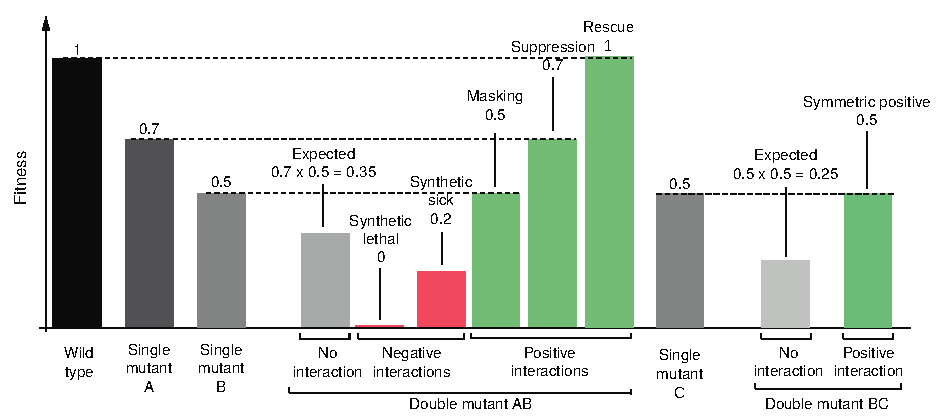
\includegraphics{Costanzo_2011_SL_mega_no_border.pdf}
    }}
   \caption[Synthetic genetic interactions]{\small \textbf{Synthetic genetic interactions.} Impact of various negative and positive \glspl{SGI}: negative interactions involve deleterious (sick) or inviable (lethal) phenotypess whereas positive interactions involve restoring viability by masking or suppressing the other mutation or complete rescue of the wildtype phenotype. Figure adapted from \citep{Costanzo2011} concerning growth viability fitness in yeast.}
\label{fig:Costanzo2011}
\end{mdframed}
\end{figure}

\subsection{Synthetic Lethal Concepts in Genetics}

\Gls{synthetic lethal} genes are generally regarded to arise due to functional redundancy. Due to the functional level of \glspl{SGI}, \gls{synthetic lethal} genes do not need directly interact, nor be expressed in the same cell or at the same developmental stage: serving related functions is sufficient to affect cell (or organism) viability and be relevant to drug-mode-of-action cancer biology. Combined loss of genes performing an essential or important function in a cell are therefore deleterious. \Gls{synthetic lethal} gene pairs are therefore pairwise essential with ``induced essentiality'': each \gls{synthetic lethal} gene becomes essential to the cell upon loss of the other.

Since \gls{synthetic lethal} gene partners can be affected by extracellular stimuli such as chemicals, essentiality of \gls{synthetic lethal} genes can be induced by the environment of a cell.  An environmental stress condition may inhibit one or the other \gls{synthetic lethal} gene, such as exposure to chemicals, in which case the \gls{synthetic lethal} partner gene is ``conditionally essential'' \citep{Hillenmeyer2008}. Thus the evolutionary rationale for the abundance of \glspl{SGI} (compared to the surprisingly low number of essential genes) in a Eukaryotic genome attributed to genetic functional redundancy and network robustness of a cell which are advantageous to survival. 

Biological functions are typically performed by a pathway of genes (or their products). Many genes of the same pathway may be fucntionally interchangable as \gls{synthetic lethal} partners of a particular gene since loss of the pathway is deleterious without the \gls{synthetic lethal} partner gene. Therefore biological pathways can be subject to induced essentiality under loss of a gene and \glspl{synthetic lethal} may occur at pathway level or in a gene regulation network. 

\subsection{Studies of Synthetic Lethality}
Genetic high-throughput screens have identified unexpected, functionally informative, and clinically relevant \gls{synthetic lethal} interactions; including \gls{synthetic lethal} partners of genes recurrently mutated in cancer or attributed to familial early-onset cancers. While screening presents an appealing strategy for \gls{synthetic lethal} discovery, computational approaches are becoming popular as an alternative or complement to experimental methods to overcome inherent bias and limitations of experimental screens. An array of recently developed computational methods \citep{Wang2013, Tiong2014, Jerby2014, Lu2015, Wappett2014} show the need for \gls{synthetic lethal} discovery in the fundamental genetics and translational cancer research community. However, existing computational methods are not suitable for queries of genomic data for interacting partners of a particular gene: they have been applied pairwise across the genome, do not have software released to apply the methodology, or lack statistical measures of error for further analysis. A robust prediction of gene interactions is an effective and practical approach at a scale of the entire genome for ideal translational applications, analysis of biological systems, and constructing functional gene networks.

\subsubsection{Synthetic Lethal Pathways and Networks}
\glspl{SGI} are very common in genomes, with 4$\times$ more interactions detected with synthetic gene array mating screens than protein-protein interactions yeast-2-hybrid studies \citep{Tong2004}. The \gls{SGI} network is scale-free with power-law vertex degree distribution and low average shortest path length (3.3) as expected for a complex biological network \citep{Barabasi2004}. Highly connected ``hub'' genes with the highest number of links (vertex degree) are functionally important with many negative \gls{SGI} hubs involved in cell cycle regulation and many positive \gls{SGI} hubs involved in translation \citep{Baryshnikova2010b, Costanzo2010}. Negative \glspl{SGI} were far more common than positive \glspl{SGI}, with synthetic gene loss being more likely to be deleterious to cell than advantageous which indicates than \glspl{synthetic lethal} may be comparably easier to detect than other \glspl{SGI}. 

Essential pathways are highly buffered with 5$\times$ more interactions than other \glspl{SGI}, consistent with strong selection for survival, as found with conditional and partial mutations in essential genes \citep{Davierwala2005}. This \gls{SGI} network had scale-free topology and rarely shared interactions with the protein-protein interaction network. These networks are related by an ``orthogonal'' relationship: shared partners in one network tend to be themselves connected directly in the other network. Essential genes were likely to have closely related functions, whereas non-essential networks were relatively more inclined to have \glspl{SGI} between distinct biological pathways. 

\subsubsubsection{Evolution of Synthetic Lethality}
There is poor conservation of specific \glspl{SGI} between \textit{S. cerevisiae} and \textit{S. pombe} with 29\% of the interactions tested in both distantly related species being conserved between them \citep{Dixon2008}. The remaining interactions show high species-specific differences; however, many of the species-specific interactions were still conserved between biological pathways, protein complexes, or protein-protein interaction modules. Similarly, conservation of pathway redundancy was also found between  Eukaryotes (\textit{S. cerevisiae}) and prokaryotes (\textit{E. coli}) \citep{Butland2008}. Negative \glspl{SGI} were more likely to be conserved between biological pathways, whereas positive \glspl{SGI} were more likely to be conserved within a pathway or protein complex \citep{Roguev2008}. 

A modest 5\% of interactions were conserved between unicellular (\textit{S. cerevisiae}) and multicellular (\textit{C. elegans}) organisms. However, the nematode \gls{SGI} network had similar scale-free topology and modularity despite differences in methodology: metazoan \gls{RNAi} screens are incomplete knockouts whereas screening null mutations is feasible in yeast \citep{Bussey2006}. The nematode \gls{SGI} screen identified network hubs with important interactions to orthologues of known human disease genes \citep{Lehner2006}. Despite the lack of direct conservation of \glspl{SGI} between yeasts and nematode worms, genetic redundancy at the gene or pathway level may yet be consistent with an induced essentiality model of \glspl{SGI} where gene functions are conserved with network restructuring over evolutionary change \citep{Tischler2008}. While nematode models are more closely related to human cells, cancer cells can present growth and viability phenotypes more comparable to yeast models. Therefore findings from both SGA and \gls{RNAi} models are relevant to understanding cellular network structure and in healthy and cancerous human cells. \gls{RNAi} has also been applied to human and mouse cancer cells in cell culture and genetic screening experiments. These findings suggest that \gls{SGI} network ``rewiring'' is a concern for identifying specific \gls{synthetic lethal} interactions in cancer and a pathway approach may be more robust in the context of evolution, patient variation, tumour heterogeneity, and disease progression.  

\subsection{Synthetic Lethal Concepts in Cancer}

Loss of function occurs in many genes in cancers including tumour suppressors and yet few interventions target such mutations compared to targeted therapies for gain of function mutation in oncogenes \citep{Kaelin2005}. \Glspl{synthetic lethal} is a powerful design strategy for therapies selective against loss of gene function with potential for application against a range of genes and diseases \citep{Kaelin2009, Fece2015}. Since \glspl{synthetic lethal} affects cellular viability by indirect functional relationships between genes, it is suitable for indirectly targeting mutations in cancers. Once \gls{synthetic lethal} partners of cancer genes are identified, targeted therapeutics can be applied against them. When genes are disrupted in cancers, the induced essentiality of \gls{synthetic lethal} partners is a vulnerability that may be exploited for anti-cancer therapy. This has the potential to be very specific against cancer cells (with the target mutation) over non-cancer cells (with a functional compensating gene). Analogous to ``oncogene addiction'', where cancer cells adapt to particular oncogenic growth signals and become reliant on them to remain viable \citep{Luo2009, Weinstein2000}, \gls{synthetic lethal} partners of inactivated tumour suppressors are required to maintain cancer cell viability and proliferation. As such cancers are subject to ``non-oncogene addiction'' and are feasible anti-cancer drug targets. 


\begin{figure}[!ht]
\begin{mdframed}
   \makebox[1 \textwidth][c]{ 
   \resizebox{0.75 \textwidth}{!}{
   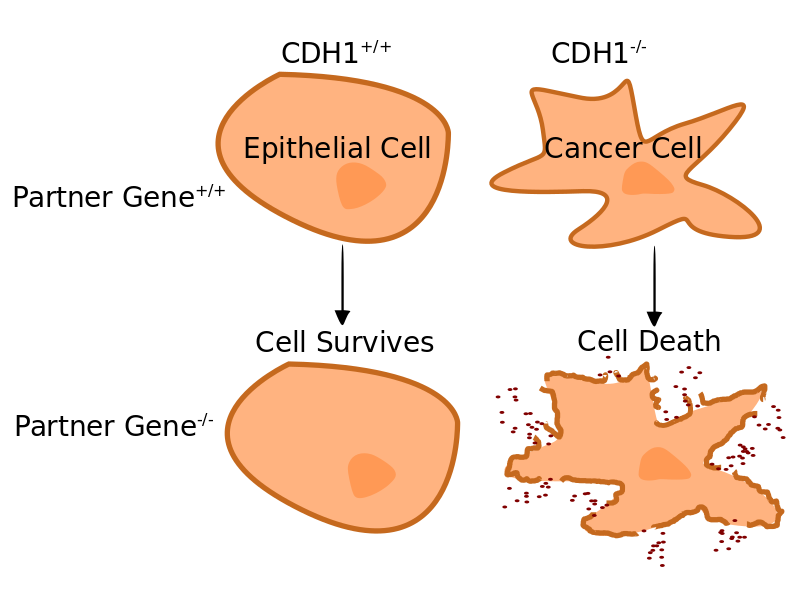
\includegraphics{SL_Concept_no_border.png}
   }}
      \caption[\Glspl{synthetic lethal} in cancer]{\small \textbf{\Glspl{synthetic lethal} in cancer.} Rationale of exploiting \glspl{synthetic lethal} for specifity against a tumour suppressor gene (e.g.,  \textit{CDH1}) while other cells are spared under the inhibition of a partner gene.}
\label{fig:SL_Concept}
\end{mdframed}
\end{figure}

The \gls{synthetic lethal} approach to cancer medicine is most amenable to loss of function mutations in tumour suppressor genes, where it would feasibly be effective against any loss of function mutation across the tumour suppressor with a viable \gls{synthetic lethal} partner gene (as shown in Figure~\ref{fig:SL_Concept}). However, the approach may also be suitable for cases where cancer cells have mutations where the normal function of the gene is disrupted such as if it were overexpression (``synthetic dosage lethality'') or if an oncogene interfered with the function of the proto-oncogenic variant such as competitive inhibition. Thus \glspl{synthetic lethal} expands the range of cancer-specific mutations feasible to target with targeted therapeutics to absence of tumour suppressor genes and distinguishing highly homologous oncogenes by functional differences by targeting their \gls{synthetic lethal} partners. 

\subsection{Clinical Impact of Synthetic Lethality in Cancer}

%Targeted therapeutics combined with the adoption of \gls{genomics} to identify mutations have begun to impact upon the clinical treatment of cancers. Early examples of targeted therapies are strikingly effective, such as vemurafenib which has shown promise against \textit{BRAF}(V600E) mutations in melanomas in clinical trials \citep{Ravnan2012} and may be widely applicable despite issues with genetic background and drug resistance \citep{Sun2014,Prahallad2012}. Meanwhile, \gls{synthetic lethal} drug design to indirectly target inactivated genes in cancer has the potential to drastically accelerate the development of precision cancer medicine \citep{Kaelin2009}.

%\Gls{synthetic lethal} interaction between \textit{\textit{PARP1}} and the tumour suppressor genes \textit{\textit{BRCA1}} and \textit{\textit{BRCA2}} has been demonstrated in cell line and mouse xenograft models, with promising results in both \gls{RNAi} and drug inhibition experiments \citep{Bryant2005,Farmer2005}. These interactions have been shown to be clinically relevant, with the \textit{\textit{PARP1}}-targeting drug olaparib exhibiting success in clinical trials involving germline and sporadic \textit{\textit{BRCA1}} or \textit{\textit{BRCA2}} mutations in both breast and ovarian cancers, and resulting in fewer adverse effects than cytotoxic chemotherapy \citep{Tutt2010,Audeh2010}. \textit{\textit{PARP1}} inhibitors have shown anti-cancer activity against mutations in other DNA repair genes such as \textit{PTEN} and have been proposed for chemopreventative applications as an alternative to prophylactic surgery for high risk individuals with germline \textit{BRCA1} or \textit{BRCA2} mutations \citep{Strom2012}. Complications were observed in clinical trials, such as acquired drug resistance, complex modifier interactions with \textit{\textit{PARP1}} inhibitors, and their application integrated with genetic tests across cancers in multiple tissues (most commonly breast and ovarian) \citep{Lord2014}. 

The \gls{synthetic lethal} interaction of \textit{BRCA1} or \textit{BRCA2} with \textit{PARP1} in breast cancer is an example of how gene interactions are important in cancer, including translation to the clinic. These genetic interactions enable specific targeting of mutations in \textit{BRCA1} or \textit{BRCA2} tumour suppressor genes with PARP inhibitors by inducing \glspl{synthetic lethal} in breast cancer \citep{Farmer2005}. PARP inhibitors are one of the first targeted therapeutics against a tumour suppressor mutation with success in clinical trials. 

\textit{BRCA1} or \textit{BRCA2} and \textit{PARP1} genes demonstrate the application of the \gls{synthetic lethal} approach to cancer therapy \citet{Ashworth2008, Kaelin2005}. \textit{BRCA1} and \textit{BRCA2} are homologous DNA repair genes, widely known as tumour suppressors; mutation carriers have substantially increased risk of breast (risk by age 70 of 57\% for \textit{BRCA1} and 59\% for \textit{BRCA2}) and ovarian cancers (risk by age 70 of 40\% for \textit{BRCA1} and 18\% for \textit{BRCA2}) \citep{Chen2007}. The \textit{BRCA1} or \textit{BRCA2} genes, which usually repair DNA or destroy the cell if it cannot be repaired, have inactivating somatic mutations in some familial and sporadic cancers. Poly-ADP-ribose polymerase (PARP) genes are tumour suppressor genes involved in base excision DNA repair. Loss of PARP activity results in single-stranded DNA breaks. However, \textit{PARP1}$^{-/-}$ knockout mice are viable and healthy indicating low toxicity from PARP inhibition \citep{Bryant2005}.  

\citet{Bryant2005} showed that \textit{BRCA2} cells were sensitive to PARP inhibition by siRNA of \textit{PARP1} or drug inhibition (which targets \textit{PARP1} and \textit{PARP2}) using Chinese hamster ovary cells, MCF7 and MDA-MB-231 breast cell lines. This effect was sufficient to kill mouse tumour xenografts and showed high specificity to \textit{BRCA2} deficient cells in culture and xenografts. \citet{Farmer2005} replicated these results in embryonic stem cells and showed that \textit{BRCA1} cells were also sensitive to PARP inhibition relative to the wild-type with siRNA and drug experiments in cell culture and drug activity against \textit{BRCA1} or \textit{BRCA2} deficient embryonic stem cell mouse xenografts. They found evidence that PARP inhibition causes DNA lesions, usually repaired in wild-type cells, which lead to chromosomal instability, cell cycle arrest, and induction of apoptosis in \textit{BRCA1} or \textit{BRCA2} deficient cells. Therefore, the pathways cooperate to repair DNA giving a plausible mechanism for combined loss as an effective anti-cancer treatment.  

Thus PARP inhibitors have potential for clinical use against \textit{BRCA1} or \textit{BRCA2} mutations in hereditary and sporadic cancers (Ashworth 2008; Kaelin2005). PARP inhibition has been found to be effective in cancer patients carrying \textit{BRCA1} or \textit{BRCA2} mutations and some other ovarian cancers, suggesting \glspl{synthetic lethal} between PARP and other DNA repair pathways \citep{Strom2012}. This supports the potential for PARP inhibition as a chemo-preventative alternative to prophylactic surgery for high risk individuals with \textit{BRCA1} or \textit{BRCA2} mutations \citep{Strom2012}. Hormone-based therapy has also been suggested as a chemo-preventative in such high risk individuals and aromatase inhibitors have completed phase I clinical trials for this purpose (Bozovic-Spasojevic2012). \citet{Strom2012} also postulate increased efficacy of PARP inhibitors in the hypoxic DNA-damaging tumour micro-environment.  

A PARP inhibitor, olaparib, showed fewer adverse effects than cytotoxic chemotherapy and anti-tumour activity in phase I trials against \textit{BRCA1} or \textit{BRCA2} deficient familial breast, ovarian, and prostate cancers \citep{Fong2009} and sporadic ovarian cancer \citep{Fong2010}. AstraZeneca has reported phase II trials showing the treatment is effective in \textit{BRCA1} or \textit{BRCA2} deficient breast \citep{Tutt2010} and ovarian cancers \citep{Audeh2010} with a favourable therapeutic window and similar toxicity between carriers of \textit{BRCA1} or \textit{BRCA2} mutations and sporadic cases. AstraZeneca announced that olaparib has begun phase III trials for breast and ovarian cancers in 2013. Mixed results in phase II trials in ovarian cancer are behind the delays addressed by retrospective analysis of the cohort subgroup with confirmed mutation of \textit{BRCA1} or \textit{BRCA2} genes in the tumour; unsurprisingly these patients, benefit most from the PARP inhibitor treatment and have increased platinum sensitivity in combination treatment. These PARP inhibitors are FDA approved for some cancers \cite{McLachlan2016}, are effective against germline and sporadic \textit{BRCA1} or \textit{BRCA2} mutations, and are a potential prevention alternative to prophylactic surgery for high risk mutation carriers \cite{Strom2012}.

This demonstrates the clinical impact of a well characterised system of \glspl{synthetic lethal} with known cancer risk genes. \Glspl{synthetic lethal} has the benefit of being effective against inactivation of tumour suppressor genes by any means, broader than targeting a particular oncogenic mutation \citep{Kaelin2005}. The targeted therapy is effective in both sporadic and hereditary \textit{BRCA1} or \textit{BRCA2} deficient tumours acting against an oncogenic molecular aberration across several tissues.  

\subsection[High{}-throughput Screening for Synthetic Lethality]{High-throughput Screening for Synthetic Lethality}

%Candidate hypothesis driven \gls{synthetic lethal} studies in cancer have been successful in some cases \citep{Farmer2005,Bryant2005,vanPel2013} but potentially meaningful \gls{synthetic lethal} interactions can also occur between unexpected pathways and with genes involved in different biological functions \citep{Costanzo2011}. Unbiased screening is therefore an appealing strategy to identify \gls{synthetic lethal} interactions, including those informative of novel biological functions, drug mode-of-action, or amenable to treatment. Current screening in cancer cell lines uses genetic or pharmacological approaches, with \gls{RNAi} or compound libraries respectively, to discover \gls{synthetic lethal} interactions \citep{Fece2015}.

%Genetic screens can facilitate the discovery of specific genes interacting with a particular disease gene, identify biomarkers for treatment response, and inform development of targeted therapies (with a known mode-of-action and anticipated mechanisms of resistance). \Gls{synthetic lethal} screens using \gls{RNAi} have been applied to many cancer genes in cell line models including \textit{\textit{VHL}} in renal cancer \citep{Jerby2014}, \textit{\textit{FH}} in renal cancer \citep{Boettcher2014}, \textit{\textit{WEE1}} in colorectal cancer \citep{Aarts2015}, and \textit{CDH1} in breast cancer \citep{Telford2015}. While some candidates identified in these screens are consistent with the literature or were successfully validated, \gls{RNAi} screens are susceptible to false positives and a large number of interaction candidates have not been tested, validated, or replicated \citep{Lu2015,Jerby2014,Boettcher2014,Azorsa2009}.

%Chemical screens are a complementary approach that can be used to screen for compounds effective against a particular mutation. While these identify lead compounds with specific activity against mutants, such screens do not ensure compounds are bioavailable, have known mode-of-action, or are selective against a particular target gene and key drug classes are not tested \citep{Fece2015,Kaelin2005,Chan2011}. Despite this, \gls{synthetic lethal} screens have become widely used for functional \gls{genomics} and translational  research to identify potential targets for drug development \citep{Fece2015,Telford2015,Jerby2014,Boettcher2014,vanderMeer2014}.

%relevance?
%%%%%%%%%%%
%Genomic and pharmacological screens are becoming widely used for biomedical research despite many potential sources of error \citep{Fece2015,Kaelin2009,Chan2011}.  Off-target effects \citep{Kaelin2005,Chan2011,Fece2015} and growth inhibition \citep{Diehl2014}, from delivery of potentially selective agents, is an issue with \gls{RNAi} experiments screening for differential viability between cell lines or treatment conditions such as \gls{synthetic lethal} screens. Mechanisms of gene inhibition, particularly transient gene knockdown in \gls{RNAi} screens, differ considerably from the behaviour inhibitors in the clinic \citep{Kaelin2009}. Screens are biased  towards genes which are amenable to inhibition, particularly chemical screens which are over-represented for gene functions with existing drugs inhibitors \citep{Chan2011}. Mutations, \gls{RNA} knockdown, and drug inhibition have different effects on gene function, so perhaps unsurprisingly, \gls{synthetic lethal} interactions often fail to replicate across experimental systems, cell lines, tissue types, or species \citep{Kaelin2009,Dixon2009}. Several alternatives have been raised to overcome some of these shortcomings of \gls{synthetic lethal} screens including genome-wide screens with episomal gene transfer \citep{Chan2011}, lentiviral \gls{RNAi} \citep{Diehl2014}, or CRISPR/\textit{Cas9} genome editing \citep{Fece2015,Shalem2015,Hart2015,Thompson2015}. However, these do not preclude the possibility of off-target effects or account for diverse genetic backgrounds or tumour heterogeneity \citep{Fece2015}.
%%%%%%%%%%%%
%% to consider (here or discussion): off-targets (even with newer tech), differences in KO mechanism -> effect, lack of reproducibility/validations of candidates


The function of signalling pathways and combinations of interacting genes are important in cancer research but classical genetics approaches have been limited to non-redundant pathways \citep{Fraser2004}. The emerging \gls{RNAi} technologies have vastly expanded the potential for studying genetic redundancy in mammalian experimental models including testing experimentally for \glspl{synthetic lethal} \citep{Fraser2004}. Identifying \glspl{synthetic lethal} is crucial to study gene function, drug mechanisms, and design novel therapies \citep{Lum2004}. Candidate selection of \gls{synthetic lethal} gene pairs relevant to cancer has shown some success but is limited because interactions are difficult to predict; they can occur between seemingly unrelated pathways in model organisms \citep{Costanzo2011}. While biologically informed hypotheses have had some success in \gls{synthetic lethal} discovery \citep{Bitler2015, Bryant2005, Farmer2005}, interactions occurring indirectly between distinct pathways would be missed \citep{Boone2007, Costanzo2011}. Scanning the entire genome for interactions against a clinically relevant gene is an emerging strategy being explored with high-throughput screens \citep{Fece2015} and computational approaches \citep{Boucher2013, vanSteen2011}.  

Experimental screening for \glspl{synthetic lethal} is an appealing strategy for wider discovery of functional interactions \textit{in vivo} despite many potential sources of error which must be considered. The \gls{synthetic lethal} concept has both genetic and pharmacological screening applications to cancer research. Genetic screens, with \gls{RNAi} to discover the specific genes involved, inform development of targeted therapies with a known mode of action, anticipated mechanisms of resistance, and biomarkers for treatment response. \gls{RNAi} is a transient knockdown of gene expression more similar to the effect of drugs than complete gene loss and makes comparison to screens in model organisms difficult \citep{Bussey2006}. The \gls{RNAi} gene knockdown process has inherent toxicity to some cells, potential off-target effects, and issues with a high false positive rate. Therefore, it is important to validate any candidates in a secondary screen and replicate knockdown experiments with a number of independent shRNAs. Alternative gene knockout procedures have also been proposed for \gls{synthetic lethal} screening including a genome-wide application of the CRISPR/Cas9/sgRNA genome editing technology \citep{Sander2014}, episomal gene transfer \citep{Vargas2004}, or \gls{RNAi} with lentiviral transfection for delivery of shRNA \citep{Telford2015}. Genetic screens have potential for quantitative gene disruption experiments to selectively target overexpressed genes in cancer via synthetic dosage lethality. While powerful for understanding fundamental cellular function, analysis of isogenic cell lines is inherently limited by assuming only a single mutation differs between them despite susceptibility to ``genetic drift'' and cannot account for diverse genetic backgrounds or tumour heterogeneity \citep{Fece2015}. Genetic screens thus identify targets to develop or repurpose targeted therapies for disease but alone will not directly identify a lead compound to develop for the market or clinical translation.  

Chemical screens are immediately applicable to the clinic by directly screening for selective lead compounds with suitable pharmacological properties. However chemical screens lack a known mode of action, may affect many targets, and screen a narrow range of genes with existing drugs. With either approach there are many challenges translating candidates into the clinic such as finding targets relevant to a range of patients, validation of targets, accounting for a range of genetic (and epigenetic) contexts or tumour micro-environment, identifying effective synergistic combinations, enhancers of existing radiation or cytotoxic treatments, avoiding inherent or acquired drug resistance, and developing biomarkers for patients which will respond to \gls{synthetic lethal} treatment, including integrating these into clinical trials and clinical practice. Identifying specific target genes is an effective way to anticipate such challenges, which can be approached with genetic screens, so we will focus on these and computational alternatives. Screening methods have proven a fruitful area of research, despite being costly, laborious, and having many different sources of error. These limitations suggest a need for complementary computational approaches to \gls{synthetic lethal} discovery.  

\subsubsection{Synthetic Lethal Screens}

Overexpression of genes is another suitable application for \glspl{synthetic lethal} since overexpressed genes cannot be distinguished from the wild-type by direct sequence specific targeted therapy. Overexpression of oncogenes, such as \textit{EGFR}, \textit{MYC}, and \textit{PIM1}, has been found to drive many cancers. \textit{PIM1} is a candidate for \gls{synthetic lethal} drug design in lymphomas and prostate cancers, where it interacts with \textit{MYC} to drive cancer growth. \citet{vanderMeer2014} performed an \gls{RNAi} screen for \glspl{synthetic lethal} between \textit{PIM1} overexpression and gene knockdown in RWPE prostate cancer cell lines. \textit{PLK1} gene knockdown and drug inhibition was effective as a specific inhibitor of \textit{PIM1} overexpressing prostate cells in cell culture and mouse tumour xenografts. \textit{PLK1} inhibition reduced \textit{MYC} expression in pre-clinical models, consistent with expression in human tumours in which \textit{PIM1} and \textit{PLK1} are co-expressed and correlated with tumour grade. Thus \gls{RNAi} screening was valuable to identify therapeutic targets and biomarkers for patient response as demonstrated with the finding of \textit{PLK1} as a candidate drug target against prostate cancer progression.  

\gls{HLRCC} is a cancer syndrome of predisposition to benign tumours in the uterus and risk of malignant cancer of the kidney attributed to inherited mutations in fumarate hydratase (\textit{FH}). \citet{Boettcher2014} performed an \gls{RNAi} screen on HEK293T renal cells for \glspl{synthetic lethal} with \textit{FH}. They found enrichment of haem metabolism (consistent with the literature) and adenylate cyclase pathways (consistent with cAMP dysregulation in \textit{FH} mutant cells). \Glspl{synthetic lethal} between \textit{FH} mutation and adenylate cyclases was validated with gene knockdown, drug experiments, and replicated across both HEK293T renal cells and VOK262 cells derived from a HLRCC patient, suggesting new potential treatments against the disease. %Therefore, \glspl{synthetic lethal} is applicable to metabolic dysregulation in cancer, consistent with the Warburg hypothesis (Warburg 1956), and successfully identifies specific anti-cancer drugs, even when the mechanism is unclear. 

Similarly, \gls{HDGC} is a cancer syndrome of predisposition to early-onset malignant stomach and breast cancers attributed to mutations in \gls{E-cadherin} (\textit{CDH1}). \citet{Telford2015} performed an \gls{RNAi} screen on MCF10A breast cells for \glspl{synthetic lethal} with \textit{CDH1}. They found enrichment of G-protein coupled receptors (GPCRs) and cytoskeletal gene functions. The results were consistent with a concurrent drug compound screen with a number of candidates validated by lentiviral shRNA gene knockdown and drug testing including inhibitors of Janus kinase, histone deacetylases, phosphoinositide 3-kinase, aurora kinase, and tyrosine kinases. Therefore the \gls{synthetic lethal} strategy has potential for clinical impact against \gls{HDGC}, with particular interest in interventions with low adverse effects for chemo-prevention, including repurposing existing approved drugs for activity against \textit{CDH1} deficient cancers.  

\gls{RNAi} screening for \glspl{synthetic lethal} is also useful for functional genetics to understand drug sensitivity. \citet{Aarts2015} screened WiDr colorectal cells for \glspl{synthetic lethal} between \textit{WEE1} inhibitor treatment and an \gls{RNAi} library of 1206 genes with functions known to be amenable to drug treatment or important in cancer such as kinases, phosphatases, tumour suppressors, and DNA repair (a pathway \textit{WEE1} regulates). Screening identified a number of \gls{synthetic lethal} candidates including genes involved in cell cycle regulation, DNA replication, repair, homologous recombination, and Fanconi anaemia. \Glspl{synthetic lethal} with cell-cycle and DNA repair genes was consistent with the literature and validation in a panel of breast and colorectal cell lines supported checkpoint kinases, Fanconi anaemia, and homologous recombination as \gls{synthetic lethal} partners of \textit{WEE1}. These results show that \glspl{synthetic lethal} can be used to improve drug sensitivity as a combination treatment, especially to exploit genomic instability and DNA repair, which are known to be clinically applicable from previous results with \textit{BRCA1} or \textit{BRCA2} genes and PARP inhibitors \citep{Lord2014}. Therefore, \textit{WEE1} inhibitors are an example of treatment which could be repurposed with the \gls{synthetic lethal} strategy. Similar findings would be valuable to clinicians as a source of biomarkers and novel treatments. While using a panel of cell lines to replicate findings across genetic background is a promising approach to ensure wide clinical application of validated \gls{synthetic lethal} partners, a computational approach may be more effective as it could account for wider patient variation than scaling up intensive experiments on a wide array of cell lines and could screen beyond limited candidates from an \gls{RNAi} library.  

Chemical genetic screens are also a viable strategy to identify therapeutically relevant \gls{synthetic lethal} interactions. \citet{Bitler2015} investigated \textit{ARID1A} mutations, aberrations in chromatin remodelling known to be common in ovarian cancers, for drug response. Ovarian RMG1 cells were screened for drug response specific to \textit{ARID1A} knockdown cells. They used \textit{ARID1A} gene knockdown for consistent genetic background, with control experiments and 3D cell culture to ensure relevance to drug activity in the tumour micro-environment. Screening a panel of commercially available drugs targeting epigenetic regulators found \textit{ESH2} methyltransferase inhibitors effective and specific against \textit{ARID1A} mutation with validation in a panel of ovarian cell lines. \Glspl{synthetic lethal} between \textit{ARID1A} and \textit{ESH2} was supported by decreases in H3K27me3 epigenetic marks and markers of apoptosis in response to \textit{ESH2} inhibitors. This was mechanistically supported with differential expression of \textit{PIK3IP1} and association of both \gls{synthetic lethal} genes with the \textit{PIK3IP1} promoter identifying the PI3K-AKT signalling pathway as disrupted when both genes were inhibited.
 %new paragraphs?
 
This successfully demonstrates the importance of \glspl{synthetic lethal} in epigenetic regulators, identifies a therapeutically relevant \gls{synthetic lethal} interaction, and shows that chemical genetic screens could model drug response and combination therapy in cancer cells. However this approach is limited to finding \gls{synthetic lethal} interactions between genes with known similar function, which may not be the most suitable for treatment. Further limiting experiments to genes with existing targeted drugs reduces the number of \gls{synthetic lethal} interactions detected, assumes the specificity of drugs to a particular target, and many of these drugs are not yet clinically available yet anyway, although they are clinical trials for other diseases or limited to access by patients from a particular countries.  

The examples above show that high-throughput screens are an effective approach to discover \glspl{synthetic lethal} in cancer with a wide range of applications. Screens are more comprehensive than hypothesis-driven candidate gene approaches and successfully find known and novel \gls{synthetic lethal} interactions with potential for rapid clinical application. They have the power to test mode of action of drugs, find unexpected \gls{synthetic lethal} interactions between pathways, or identify effective treatment strategies without needing a clear mechanism. However, \gls{synthetic lethal} screens are costly, labour-intensive, error-prone, and biased towards genes with effective \gls{RNAi} knockdown libraries. Limited genetic background, lethality to wild-type cell during gene knockdown, off-target effects, and difficultly replicating \glspl{synthetic lethal} across different cell lines, tissues, laboratories, or conditions stems from a high false positive rate and a lack of standardised thresholds to identify \glspl{synthetic lethal} in a high-throughput screen. Therefore there is a need for replication, validation, and alternative approaches to identify \gls{synthetic lethal} candidates. Varied conditions between experimental screens and differences between \gls{RNAi} and drug screens renders meta-analysis ineffective.

Genome-scale \gls{synthetic lethal} experiments (across gene pairs) are not feasible, even in model organisms, and they typically focus on specific gene candidates or the partners of a gene of interest (such as importance in health). Therefore a computational approach is more suitable for this task and may further augment experimental screening to replicate screen candidates beyond experimental models.  

\subsection[Computational Prediction of Synthetic Lethality]{Computational Prediction of Synthetic Lethality}

%Computational approaches to identifying \gls{synthetic lethal} interactions are rapidly developing into a feasible addition to genomic screens due to the low cost, reliable automated reproducible workflows, ability to account for distinct genetic backgrounds, and lack of off-target effects or bias towards particular genes \citep{Boucher2013, Thompson2015}. 
%%%%%%%%relevance
%\Gls{synthetic lethal} prediction has been widely explored in model organisms - a key example is the task of inferring the entire gene network from incomplete \gls{synthetic lethal} networks and functional \gls{genomics} data in \textit{Saccharomyces cerevisiae} \citep{Boucher2013}. However, \gls{synthetic lethal} interactions are difficult to reproduce across species \citep{Dixon2009,Lehner2006}, not all of the data types used for prediction of \gls{synthetic lethal} interactions in available in humans, and the methods assuming conserved network structure may not be applicable to unstable cancer systems. Computational approaches to discovery of \gls{synthetic lethal} interactions tailored to mammals, or specifically to human cancers, are therefore needed for applicable results. However, many existing computational approaches are difficult to apply to novel genes having been trained on known gene functions, using complex machine learning methods, or are over-represented for genes where single gene aberrations have large effects on cellular phenotypes such as \textit{\textit{TP53}} or \textit{AKT}.
%%%%%%% join to next subsubsubsection
%Analysis of gene expression is an appealing strategy for discovery of \gls{synthetic lethal} interactions in cancer due to the widespread availability of data for different cancers, lack of bias towards well characterised genes, and potential further use for expression of interacting partners as biomarkers for treatment with drugs designed to exploit them.

%A recent example of a computational tool for identification of \gls{synthetic lethal} interactions using gene expression analysis is the \gls{DAISY} methodology \citep{Ryan2014,Crunkhorn2014}, which combines predictions from patient samples  of The Cancer Genome Atlas (\gls{TCGA}), cell lines of the \gls{CCLE}, and \gls{RNAi} validation experiments \citep{Jerby2014}. The predictors of \glspl{synthetic lethal} were genomic `survival of the fittest' (using DNA copy number and somatic mutation in patient and cell lines data), `functional examination' of gene essentiality (using \gls{RNA} interference data in cell cell lines), and pairwise `gene co-expression' (in cell lines).

%%%%%%%% edit to tone down anti-\gls{DAISY} message  restructure subsubsubsections to fewer ideas apiece
%As a proof-of-concept, \gls{DAISY} demonstrates the potential of \gls{bioinformatics} approaches to generate \gls{synthetic lethal} candidates against the tumour suppressor \textit{\textit{VHL}} in a renal cancer cell line, along with reasonable statistical performance and generalisation to gene essentiality, genetic dosage, or drug analyses \citep{Jerby2014}. However, \gls{DAISY} partners of \textit{\textit{VHL}} showed only modest 4$\times$ over-represent\-ation in validated shRNA screening than a screen of random genes and the method has not been widely adopted in studies of other cancer genes.
%%criticism of \gls{DAISY} moved to discussion

%An alternative to the approach is the use of `cancer genome evolution' to predict \gls{synthetic lethal} genes from their behaviour in \gls{genomics} data\citep{Lu2015}, as the induced essentiality of remaining \gls{synthetic lethal} partners takes effect in the tumour progression. Lu \textit{et al.} \citep{Lu2015} postulate that, in response to loss of a gene function, a tumour would would either resist by maintaining low expression or compensate by increasing the activity of \gls{synthetic lethal} partner genes. This model predicted far more genes than previous attempts at discovery of \gls{synthetic lethal} interactions, performed well at a genome-wide scale, and produced a higher 14$\times$ over-represent\-ation of validated \gls{synthetic lethal} pairs. While Lu \textit{et al.} \citep{Lu2015} provide a comprehensive list of their strongest candidate \gls{synthetic lethal} pairs across cancer types, these do not include \textit{CDH1}, thus there remains a need for computational predictions for this gene and a tool other researchers may use for similar screen triage purposes against a candidate gene in a specific cancer.  


%% (Re)move the below subsubsubsection? Too negative / irrelevant?
%These prior approaches used complex cutting-edge machine learning techniques which may be difficult for the biological community to adopt and DNA copy number which may not be available for many  applications \citep{Jerby2014, Lu2015}. %% may be speculation
%Here, we present a \gls{synthetic lethal} analysis based solely on gene expression data which could feasibly be applied to studies of other genes to utilise the large number of samples collected for many genes in diseases such as cancers.  We use the example of \textit{CDH1} as a tumour suppressor gene in breast cancer samples from \gls{TCGA} \citep{TCGA2012} to highlight the importance of \gls{synthetic lethal} interactions, potential relationships between them, and the biological pathways involved.
%R code for our \gls{synthetic lethal} analysis will be available on our \href{https://github.com/TomKellyGenetics/slipt}{GitHub repository} as an R package. 

\subsubsection{Bioinformatics Approaches to Genetic Interactions}

Prediction of gene interaction networks is a feasible alternative to high-throughput screening with biological importance and clinical relevance. There are many existing methods to predict gene networks, as reviewed by \citet{vanSteen2011} and \citet{Boucher2013} and summarised in Table~\ref{tab:methods_model}. However, many of these methods have limitations including the requirement for existing \gls{SGI} data, several data inputs, and reliability of gene function annotation. Many of the existing methods also assume conservation of individual interactions between species, which has been found not to hold in yeast studies \citep{Dixon2008}. Tissue specificity is important in gene regulation and gene expression, which are used as predictors of genetic interaction. However, tissue specificity of genetic interactions cannot be explored in yeast studies and has not been considered in many studies of multicellular model organisms, human networks, or cancers. Similarly, investigation into tissue specificity of protein-protein interactions (PPIs) , an important predictor of genetic interactions, is difficult given that high-throughput two-hybrid screens occur out of cellular context for multicellular organisms.  

\begin{table}[!ht]
\caption{Methods for Predicting Genetic Interactions}
\label{tab:methods_model}
\makebox[\textwidth][c]{
\resizebox{1.15 \textwidth}{!}{
%\setlength\LTleft{0pt}
%\setlength\LTright{0pt}
\begin{tabular}{lllll}

\multicolumn{1}{l}{\textbf{Method}} &
\multicolumn{1}{l}{\textbf{Input Data}} &
\multicolumn{1}{l}{\textbf{Species}} &
\multicolumn{1}{l}{\textbf{Source}} &
\multicolumn{1}{l}{\textbf{Tool Offered}} \\ \hline
\cellcolor{black!10}\color{black} %\cellcolor[rgb]{0.8509804,0.8862745,0.9529412}
\textcolor{black}{Between Pathways Model} &
\cellcolor{black!10}\color{black} PPI, \gls{SGI} &
\cellcolor{black!10}\color{black}
\textit{\textcolor{black}{S. cerevisiae}} &
\cellcolor{black!10}\color{black}
\citet{Kelley2005} &
\cellcolor{black!10}~
\\
Within Pathways Model &
PPI, \gls{SGI} &
\textit{S. cerevisiae} &
\citet{Kelley2005} &
~
\\
\cellcolor{black!10}\color{black}
\textcolor{black}{Decision Tree} &
\cellcolor{black!10}\color{black} PPI,
expression, phenotype &
\cellcolor{black!10}\color{black}
\textit{\textcolor{black}{S. cerevisiae}} &
\cellcolor{black!10}\color{black}
\citet{Wong2004} &
\cellcolor{black!10}\color{black} 2
Hop\\
Logistic Regression &
\gls{SGI}, PPI, co-expression, phenotype &
\textit{C. elegans} &
\cite{Zhong2006} &
Gene Orienteer\\
\cellcolor{black!10}\color{black}
\textcolor{black}{Network Sampling} &
\cellcolor{black!10}\color{black} \gls{SGI}, PPI, GO
&
\cellcolor{black!10}\color{black}
\textit{\textcolor{black}{S. cerevisiae}} &
\cellcolor{black!10}{
\begin{tabular}{@{\hskip0pt}l@{\hskip0pt}}\color{black}\citet{LeMeur2008} \\ \color{black}\citet{LeMeur2014}\end{tabular}}
&
\cellcolor{black!10}\color{black}
SLGI(R)\\
Random Walk &
GO, PPI, expression &

\begin{tabular}{@{\hskip0pt}l@{\hskip0pt}}\textit{S. cerevisiae} \\ \textit{C. elegans}\end{tabular}
 &
\citet{Chipman2009} &
~
\\
\cellcolor{black!10}\color{black}
\textcolor{black}{Shared Function} &
\cellcolor{black!10}\color{black}
Co-expression, PPI, text mining, phylogeny &
\cellcolor{black!10}\color{black}
\textit{\textcolor{black}{C. elegans}} &
\cellcolor{black!10}\color{black}
\citet{Lee2010b} &
\cellcolor{black!10}\color{black}
WormNet\\
Logistic Regression &
Co-expression, PPI, phenotype &
\textit{C. elegans} &
\citet{Lee2010a} &
GI Finder\\
\cellcolor{black!10}\color{black}
\textcolor{black}{Jaccard Index} &
\cellcolor{black!10}\color{black} GO, \gls{SGI},
PPI, phenotype &
\cellcolor{black!10}\color{black} Eukarya &
\cellcolor{black!10}\color{black}
\citet{Hoehndorf2013} &
\cellcolor{black!10}~
\\
\iffalse
Bimodal Statistics &
~
 &
~
 &
\cite{Wappett2014} &
\gls{BiSEp}(R)\\
\cellcolor{black!10}\color{black}
\textcolor{black}{Machine Learning} &
\cellcolor{black!10}~
 &
\cellcolor{black!10}~
 &
\cellcolor{black!10}
\begin{tabular}{@{\hskip0pt}l@{\hskip0pt}}\color{black} Discussed by \citep{Babyak2004} \\and \citet{Lee2009} \end{tabular}

 &
\cellcolor{black!10}~
\\
\begin{tabular}{@{\hskip0pt}l@{\hskip0pt}}\color{black} Machine Learning \\as discussed by \citet{Wu2014}  \end{tabular}
&
~
 &
~
 &

\begin{tabular}{@{\hskip0pt}l@{\hskip0pt}}
\citet{Qi2008} \\
\citet{Paladugu2008} \\
\citet{Li2011}
\end{tabular}
&
~
\\
\fi
\cellcolor{black!5}\color{black}
\textcolor{black}{Machine Learning} &
\cellcolor{black!5}~
 &
\cellcolor{black!5}~
 &
\cellcolor{black!5}\color{black}
\citet{Pandey2010} &
\cellcolor{black!5}\color{black} MNMC\\
\rowcolor{black!10}
Machine Learning Meta-Analysis &
~
 &
~
 &
\cite{Wu2014} &
MetaSL\\
\cellcolor{black!5}{\color{black}
\begin{tabular}{@{\hskip0pt}l@{\hskip0pt}}
\textcolor{black}{Flux Variability Analysis} \\
\textcolor{black}{Flux Balance Analysis} \\
\textcolor{black}{Network Simulation}
\end{tabular}
} &
\cellcolor{black!5}\color{black} Metabolism &
\cellcolor{black!5}{\color{black}

\begin{tabular}{@{\hskip0pt}l@{\hskip0pt}}
\textit{\textcolor{black}{E. coli}} \\
\color{black} \textit{\textcolor{black}{M. pneumoniae}}
\end{tabular}
} &
\cellcolor{black!5}\color{black}
\citet{Guell2014} &
\cellcolor{black!5}~
\\ \hline
\end{tabular}
}
}
\end{table}

\begin{table*}[!ht]
\caption{Methods for Predicting Synthetic Lethality in Cancer}
\label{tab:methods_SL}
%\begin{center}
\resizebox{ \textwidth}{!}{
\begin{tabular}{llll}
\multicolumn{1}{m{4.421cm}}{\cellcolor{white}\bfseries\color{black}
Method} &
\multicolumn{1}{m{2.342cm}}{\cellcolor{white}\bfseries\color{black}
\textcolor{black}{Input Data}} &
\multicolumn{1}{m{4.552cm}}{\cellcolor{white}\bfseries\color{black}
Source} &
\cellcolor{white}\bfseries\color{black} Tool Offered\\
\hline
\cellcolor{black!10}\color{black}
\textcolor{black}{Network Centrality} &
\cellcolor{black!10}\color{black} protein-protein interactions &
\cellcolor{black!10}\color{black}
\citet{Kranthi2013} &
\cellcolor{black!10}~
\\
Differential Expression &
\begin{tabular}{@{\hskip0pt}l@{\hskip0pt}}
Expression \\
Mutation
\end{tabular}
&
\citet{Wang2013} &
~
\\
\cellcolor{black!10}{\color{black}

\begin{tabular}{@{\hskip0pt}l@{\hskip0pt}}
\textcolor{black}{Comparative \Gls{genomics}} \\
\color{black} \textcolor{black}{Chemical-\Gls{genomics}}
\end{tabular}
}
 &
\cellcolor{black!10}

\begin{tabular}{@{\hskip0pt}l@{\hskip0pt}}
Yeast synthetic gene interactions\\
Homology
\end{tabular}
 &
\cellcolor{black!10}\color{black}
\citet{Heiskanen2012} &
\cellcolor{black!10}~
\\
Comparative \Gls{genomics} &
\begin{tabular}{@{\hskip0pt}l@{\hskip0pt}}
Yeast synthetic gene interactions \\
Homology
\end{tabular}
 &
\citet{Deshpande2013} &
~
\\
%\cellcolor{black!10}\color{black}
%\textcolor{black}{Genome Evolution} &
%\cellcolor{black!10}~
% &
%\cellcolor{black!10}\color{black}
%\citet{Lu2013} &
%\cellcolor{black!10}~
%\\
\rowcolor{black!10}

Machine Learning &
~
&
\begin{tabular}{@{\hskip0pt}l@{\hskip0pt}}\color{black} Discussed by \citet{Babyak2004} \\and \citet{Lee2009} \end{tabular}

 &
~
\\
\cellcolor{black!5}\color{black}
\textcolor{black}{Differential Expression} &
\cellcolor{black!5}Expression
 &
\cellcolor{black!5}\color{black}
\citet{Tiong2014} &
\cellcolor{black!5}~
\\
\rowcolor{black!10}
Literature Database &
~
 &
\citet{Li2014} &
Syn-Lethality\\
\cellcolor{black!5}\color{black}
\textcolor{black}{Meta-Analysis} &
\cellcolor{black!5}\color{black}
\begin{tabular}{@{\hskip0pt}l@{\hskip0pt}}
Meta-Analysis \\
Machine Learning
\end{tabular}
 &
\cellcolor{black!5}\color{black}
\citet{Wu2014} &
\cellcolor{black!5}\color{black}
MetaSL\\
\rowcolor{black!10}
Pathway Analysis &
~
 &
\citet{Zhang2015} &
~
\\
\cellcolor{black!5}\color{black}
\textcolor{black}{Protein Domains} &
\cellcolor{black!5}\color{black} Homology &
\cellcolor{black!5}\color{black}
\citet{Kozlov2015} &
\cellcolor{black!5}~
\\
\rowcolor{black!10}
\begin{tabular}{@{\hskip0pt}l@{\hskip0pt}}
Data-Mining \\
Machine Learning
\end{tabular}
 &
\begin{tabular}{@{\hskip0pt}l@{\hskip0pt}}
Expression \\
Somatic mutation and DNA CNV \\
siRNA in cell lines
\end{tabular}
 &
\begin{tabular}{@{\hskip0pt}l@{\hskip0pt}}
\citet{Jerby2014}\\
\citet{Ryan2014} \\
\citet{Crunkhorn2014} \\
\citet{Lokody2014}\end{tabular}

&
\acrshort{DAISY} (method)\\
\cellcolor{black!5}{\color{black}

\begin{tabular}{@{\hskip0pt}l@{\hskip0pt}}
\textcolor{black}{Genome Evolution} \\
{\color{black} \textcolor{black}{Hypothesis Test}} \\
\color{black} \textcolor{black}{Machine Learning}
\end{tabular}
} &
\cellcolor{black!5}{
\begin{tabular}{@{\hskip0pt}l@{\hskip0pt}}
Expression \\
DNA CNV \\
Known SL
\end{tabular}
} &
\cellcolor{black!5}\color{black}
\begin{tabular}{@{\hskip0pt}l@{\hskip0pt}}
\citet{Lu2013} \\
\citet{Lu2015}
\end{tabular}
&
\cellcolor{black!5}~
\\
\rowcolor{black!10}\color{black}
\begin{tabular}{@{\hskip0pt}l@{\hskip0pt}}
\textcolor{black}{Bimodality}
\end{tabular}
&

\begin{tabular}{@{\hskip0pt}l@{\hskip0pt}}
Expression \\
DNA CNV \\
Somatic Mutation
\end{tabular}
&
\color{black}
\begin{tabular}{@{\hskip0pt}l@{\hskip0pt}}
\citet{Wappett2014} \\
\citet{Wappett2016}
\end{tabular}
&
\gls{BiSEp}
\\
\rowcolor{black!5}
Directional Chi-Square &
\begin{tabular}{@{\hskip0pt}l@{\hskip0pt}}
Expression (microarray) \\
Somatic mutation
\end{tabular}
 &
\begin{tabular}{@{\hskip0pt}l@{\hskip0pt}}
Kelly, S. T., Guilford, P. J., and Black, M. A. \\
Dissertation (Kelly, 2013) and developed here \\
\end{tabular}
&
SLIPT\\
\hline
\end{tabular}
}
%\end{center}
\end{table*}

There are a number of existing computational methods for predicting \gls{synthetic lethal} gene pairs in humans with a specfic interest in cancer (as summarised in~\ref{tab:methods_SL}). While these demonstrate the power and need for predictions of \glspl{synthetic lethal} in human and cancer contexts, limitations of previous methods could be met with a different approach. Existing computational approaches to \gls{synthetic lethal} prediction are often difficult to interpret, replicate for new genes, or are reliant on data types not available for a wider range of genes to test.  

\subsubsection{Comparative Genomics}

A comparative \gls{genomics} approach by \citet{Deshpande2013} used the results of well characterised high-throughput mutation screens in \textit{S. cerevisiae} as candidates for \glspl{synthetic lethal} in humans \citep{Baryshnikova2010a, Costanzo2010, Costanzo2011, Tong2001, Tong2004}. Yeast \gls{synthetic lethal} partners were compared to human orthologues to find cancer relevant \gls{synthetic lethal} candidate pairs with direct therapeutic potential. Proposed as a complementary approach to siRNA screens, approximately 24,000 of the 116,000 negative \glspl{SGI} in yeast \citep{Costanzo2011} were matched to human orthologues, with over 500 involving a cancer gene \citep{Futreal2004}. Under strict criteria of one-to-one orthologues, large effect size and significant interaction in yeast data ($\epsilon < -0.2$, $p < 0.05$), 1,522 interactions were identified with 70 involving cancer genes. Of the 21 gene interactions tested with pairs of siRNA in IMR1 fibroblast cells, 6 exhibited \gls{synthetic lethal} effects. The two strongest interactions (\textit{SMARCB1} with \textit{PSMA4} and \textit{ASPSCR1} with \textit{PSMC2}) were successfully validated by protein analysis of human cells and replication with tetrad analysis for yeast orthologues.

Another approach to systematic \glspl{synthetic lethal} discovery specific to human cancer (in contrast to the plethora of yeast \glspl{synthetic lethal} data) was to build a database as done by \citet{Li2014}. In their relational database, called ``Syn-lethality'', they have curated both known experimentally discovered \gls{synthetic lethal} pairs in humans (113 pairs) from the literature and those predicted from \glspl{synthetic lethal} between orthologous genes in \textit{S. cerevisiae} yeast (1114 pairs). This knowledge-based database is the first dedicated to human cancer \gls{synthetic lethal} interactions and integrates gene function annotation, pathway and molecular mechanism data with experimental and predicted \gls{synthetic lethal} gene pairs. This combination of data sources is intended to tackle the trade-off between more conclusive \gls{synthetic lethal} experiments in yeast and more clinically relevant \gls{synthetic lethal} experiments in human cancer models, such as \gls{RNAi}, especially when high-throughput screens are costly and prone to false positives in either system and difficult to replicate across gene backgrounds. This database centralises a wealth of knowledge scattered in the literature including cancer relevant genes (\textit{BRCA1}, \textit{BRCA2}, \textit{PARP1}, \textit{PTEN}, \textit{VHL}, \textit{MYC}, \textit{EGFR}, \textit{MSH2}, \textit{KRAS}, and \textit{TP53}) and is publicly available as a Java App. These included the previously mentioned interactions of \textit{BRCA1} and \textit{BRCA2} with \textit{PARP1} and \textit{TP53} with \textit{WEE1} and \textit{PLK1}. However, the computational methodology was not released, so it is not possible to replicate their results, nor to add to the findings with new datasets, which are limited to 647 human genes. Suggested future directions were promising, such as constructing networks of known \glspl{synthetic lethal}, applying known \glspl{synthetic lethal} to cancer treatment, data mining, replicating the approach for \glspl{synthetic lethal} in model organisms, signalling pathways, and developing a complete global network in human cancer or yeast (both of which are still incomplete with experimental data), some of which has been implemented in ``SynLethDB'' \citep{Guo2016}.  


\begin{table*}[!ht]
\caption[Methods used by \citet{Wu2014}]{Machine Learning Methods used by \citet{Wu2014}}
\label{tab:methods_meta}
%\begin{center}
\resizebox{ \textwidth}{!}{
\begin{tabular}{lll}
\multicolumn{1}{m{4.421cm}}{\cellcolor{white}\bfseries\color{black}
Method} &
\multicolumn{1}{m{4.552cm}}{\cellcolor{white}\bfseries\color{black}
Source} &
\cellcolor{white}\bfseries\color{black} Tool Offered\\
\hline
\cellcolor{black!10}\color{black}
\textcolor{black}{Random Forest} &
\cellcolor{black!10}{\color{black}
\citet{Breiman2001}
}
&
\cellcolor{black!10}~\\
\begin{tabular}{@{\hskip0pt}l@{\hskip0pt}}
Random Forest \\
J48 (decision tree) \\
Bayes (Log Regression) \\
Bayes (Network) \\
PART (Rule-based) \\
RBF Network \\
Bagging / Bootstrap \\
Classification via Regression
\end{tabular}
&
\citet{Hall2009}
~
 &
WEKA\\
\cellcolor{black!10}\textcolor{black}{Support Vector Machine (Linear)} &
\cellcolor{black!10}\color{black}
\citet{Vapnik1995} &
\cellcolor{black!10}~
\\
Support Vector Machine (RBF -- Gaussian) &
\citet{Joachims1999} &
~
\\
\cellcolor{black!10}\color{black}
\textcolor{black}{Multi-Network Multi-Class (MNMC)} &
\cellcolor{black!10}\color{black}
\citet{Pandey2010} &
\cellcolor{black!10}~
\\
MetaSL (Meta-Analysis) &
\citet{Wu2014} &
MetaSL\\
\hline
\end{tabular}
}
%\end{center}
\end{table*}

Machine learning approaches have also been proposed for \gls{synthetic lethal} discovery \citep{Babyak2004, Lee2009}. Due to concerns that these may be subject to overfitting or noise, \citet{Wu2014} developed a meta-analysis method (based on the machine learning methods in Table~\ref{tab:methods_meta}) for \gls{synthetic lethal} gene pairs relevant to developing selective drugs against human cancer, building upon their previous database \citep{Li2014}. They used training data of 10,885 \gls{synthetic lethal} interactions from yeast experiments of which 7347 occurred between the 5,504 non-essential genes. Their ``metaSL'' approach utilises genomic, proteomic and annotation data (including GO terms \cite{Ashburner2000}, PPI, protein complexes, and biological pathway) with strong statistical performance in yeast data (\gls{AUROC} of 0.871). The predicted orthologous \gls{synthetic lethal} partners in human data were not experimentally validated but several would be relevant to cancer such as \textit{EGFR} with \textit{PRKCZ}. They note that computational approaches scale-up across the genome at lower cost than experimental screen and share their most supported interactions online. However, the method is not available for analysis of other genes studied by the cancer research community. While machine learning has great potential as a predictor, the results vary greatly depending on the predictive features selected and it is not clear which threshold should be used to report reliably detected genes. Syn-Lethality \citep{Li2014} and MetaSL \citep{Wu2014} demonstrate the value of computational approaches to \glspl{synthetic lethal} but omit many genes of importance in cancer, such as \textit{CDH1}, and there remains a need to enable biological researchers to query such genes in a particular tissue or genetic background. 

There is also concern for analyses based on yeast data that many \gls{synthetic lethal} interactions may not be conserved between species \citet{Dixon2009a}, although interactions between pathways may be more comparable. It is unsurprising that many of the interactions identified were not experimentally validated. There have been many gene duplications in the separate evolutionary histories of humans and yeast which may lead to differences in genetic redundancy. Yeast are not an ideal human cancer model because they are do not have tissue specificity, multicellular gene regulation, or orthologues to a number of known cancer genes such as p53. Although these studies have tried to anticipate these issues with stringent criteria such as requiring one-to-one orthologues, there remains the possibility that changes in gene function may affect whether these are solely redundant such as if functions had coevolved without sequence homology. Many genes will also be excluded since they lack homologues in yeast, the corresponding experimental data, or having paralogues in either species. Thus conservation of yeast interactions is not an ideal strategy and analysis of human data directly for comparison with human experimental data will be the focus of this thesis. 

\subsubsection{Analysis and Modelling of Protein Data}

\citet{Kranthi2013} took a network approach to discovery of \gls{synthetic lethal} candidate selection applying the concept to ``centrality'' to a human PPI network involving interacting partners of known cancer genes. The effect of removing pairs of genes on connectivity of the network was used as a surrogate for viability which is supported by observations that the PPI and \gls{synthetic lethal} networks are orthogonal in \textit{S. cerevisiae} studies \citep{Tong2004}. They showed that the human cancer protein interaction network (of 1539 proteins and 6471 interactions) exhibits the power law distribution expected of a scale-free \gls{synthetic lethal} network with high connectivity (average vertex degree of 23.67 and network efficiency of 0.2952). Their top 100 candidate interactions included interactions of the tumour suppressor \textit{TP53} with \textit{BRCA1}, \textit{CDKNA1}, \textit{CDKNA2}, \textit{MET}, and \textit{RB1} which have been detected by prior studies. The gene pairs were often observed to be in the same or a plausible compensatory pathway. Thus the network structure is important in the biological functions of cancers and could be exploited for targeting \textit{TP53} loss of function mutations. 

However, their approach was limited to known cancer genes and is not applicable to genes that do not have PPI data. Other nucleotide sequencing data types are more commonly available for cancer studies at a genomic scale. Of further concern is that the results were enriched for p53 \gls{synthetic lethal} partners which is relevant to many cancer researchers but this genome-wide approach did not detect many other cancer genes due to multiple testing. This enrichment may be due to the known drastic effect of removing p53 itself from the network as a master regulator, cancer driving tumour suppressor gene, and highly connected network ``hub''. The focus on cancer genes is useful for translation into therapeutics but does not account for variable genetic backgrounds or effect of protein removal on the whole cellular network.  

Focusing on the potential for \glspl{synthetic lethal} to be an effective anti-cancer drug target, \citet{Zhang2015} used modelling of signalling pathways to identify \gls{synthetic lethal} interactions between known drug targets and cancer genes by simulating gene knockdowns. A computational approach was applied to avoid the limitations of experimental \gls{RNAi} screens such as scale, instability of knockdown, and off-target effects. This `hybrid' method of a data-driven model and known signalling pathways showed potential as a means to predict cell death in single and combination gene knockouts. They used time series protein phosphorylation data \citep{Lee2012} for 28 signalling proteins and \gls{GO} (GO) pathways \citet{Ashburner2000, Blake2015}. This approach successfully detected many known essential genes in the human gene essentiality database, known \gls{synthetic lethal} partners in the Syn-Lethality database \citep{Li2014}, and predicted novel \gls{synthetic lethal} gene pairs. The strongest essential genes in single knockdowns were \textit{AKT}, \textit{TP53}, \textit{CHK1}, \textit{S6K1}, and \textit{CYCLIND1}. Pairwise knockdowns identified 252 candidate \gls{synthetic lethal} interactions including \textit{TP53} with \textit{CHK1}, \textit{S6K1}, \textit{WEE1}, \textit{CYCLIND1}, and \textit{CASP9}; \textit{AKT} with \textit{WEE1}; and \textit{CDK1} with \textit{CYCLIND1}. These novel results contained many \textit{TP53} and AKT \gls{synthetic lethal} partners, genes known to be important in many cancers, however these also have a severe impact on the signalling pathways in their essentiality analysis of single gene disruptions and large phenotypic changes in cancer. This approach is amenable to detect functionally related pathways and protein complexes across the molecular function, cellular component, and biological process annotations provided by GO. The results were consistent with the experimental results in the literature but the novel \gls{synthetic lethal} interactions have yet to be validated. While the mathematical reasoning and algorithms are given, the code was not released to replicate the findings or apply the methodology beyond the signalling pathways analysed by \citet{Zhang2015}. While this is an interesting approach, the analysis of this thesis will focus on gene expression and \gls{RNAi} data which is available to test a wider range of candidate gene pairs.

%The authors note limitations as directions for further research including the potential of their method to detect mechanisms, types of interactions, impact of activation or inhibition of proteins, and improve performance with a Boolean network or differential equation approach, all of which have been claimed but not shown. Further, this approach is limited by existing pathway data with limited scale, scope, and reliability coming from a range of sources. So far, modelling has been restricted to signalling pathways which are immediately applicable to cancer; while important, the approach lacks broader application to other diseases and pathway types. Zhang et al. (2015) also lack validation, replication, or application of findings and are heavily reliant on existing literature for testing their predictions.  

\subsubsection{Differential Gene Expression}

Differential gene expression has been explored to predict \gls{synthetic lethal} pairs in cancer which would be widely applicable due to the availability of public gene expression data for a large number of samples and cancer types. \citet{Wang2013} found differentially expressed genes (by the t-test, adjusted by FDR) between tumours with or without functional p53 mutations in \gls{TCGA} \citep{TCGA2008GBM} and \gls{CCLE} \citep{Barretina2012} \gls{RNA-Seq} gene expression data as candidate \gls{synthetic lethal} partner pathways of p53. They identified 2, 8, and 21 candidate \gls{synthetic lethal} partner genes in 3 microarray datasets from the NCI60 cell lines, 31 partner genes from the \gls{CCLE} \gls{RNA-Seq} data, and 50 in \gls{TCGA} \gls{RNA-Seq} data. \textit{PLK1} was replicated across 4 of these analyses and 17 other genes were replicated across 2 analyses (including \textit{MTOR}, \textit{PLK4}, \textit{MAST2}, \textit{MAP3K4}, \textit{AURKA}, \textit{BUB1} and 6 CDK genes) with many playing a role in cell cycle regulation. This was supported by a drug sensitivity experiment on the NCI60 cell lines which found that cells which lacked functional p53 were more sensitive to paclitaxel (which targets \textit{PLK1}, \textit{AURKA}, and \textit{BUB1}). This demonstrated the potential of gene expression as a surrogate for gene function and use of public genomic data to predict \gls{synthetic lethal} gene pairs in cancer. \citet{Wang2013} advocated for pre-screening of expression profiles to augment future \gls{RNAi} screens. However, the analyses were limited to kinase genes and focused on currently druggable genes, lacking wider application of \gls{synthetic lethal} prediction methodology. This approach may not be feasible or applicable in cancer genes with a lower mutation rate than p53.  

\citet{Tiong2014} also investigated gene expression as a predictor of synthetic lescale-freethal pairs with colorectal cancer microarrays from a Han Chinese population with a sample size of 70 tumour and 12 normal tissue samples. Simultaneously differentially expression of ``tumour dependent'' gene pairs (which includes co-expression) between cancer and normal tissue was used to rank 663 candidate \gls{synthetic lethal} interactions identified in cell line siRNA experiments. Of the top 20 genes, 17 were tested for testing differential expression at the protein level with immunohistochemistry staining and correlation with clinical characteristics, with 11 pairs exhibiting synergistic effects. Some of the predicted \gls{synthetic lethal} pairs were consistent with the literature (including \textit{TP53} with \textit{S6K1} and partners of \textit{KRAS},  \textit{PTEN}, \textit{BRCA1}, and \textit{BRCA2}) and two novel \gls{synthetic lethal} interactions (\textit{TP53} with \textit{CSNK1E} and \textit{CTNNB1}) were validated in pre-clinical models. This serves a valuable proof-of-concept for integration of \textit{in silico} approaches to \gls{synthetic lethal} discovery in cancer demonstrating it's utility to triage and identify \gls{synthetic lethal} partners of p53 applicable to colorectal tissues. Although the experimental work was the focus of the paper, these findings show that \gls{bioinformatics} \gls{synthetic lethal} candidates can be validated in patient tissue samples (from a non-caucasian population) to find those applicable to colorectal cancers.

\subsubsection{Data Mining and Machine Learning}

\glsreset{DAISY}

Recognising the utility of \glspl{synthetic lethal} to drug inhibition and specificity of anti-cancer treatments, \citet{Jerby2014} also saw the need for effective prediction of gene essentiality and \glspl{synthetic lethal} to augment experimental studies of SL. They developed the \gls{DAISY}, a data-driven approach for genome-wide analysis of \glspl{synthetic lethal} in public cancer \gls{genomics} data from \gls{TCGA} and \gls{CCLE}  \citep{Barretina2012}. \gls{DAISY} is intended to predict the candidate \gls{synthetic lethal} partners of a query gene such as genes recurrently mutated in cancer.  

\citet{Jerby2014} combined a computational approach to triage candidates with a conventional \gls{RNAi} screen to validate \gls{synthetic lethal} partners. They screened a selection of computationally predicted candidates and randomly selected genes with \gls{RNAi} against \textit{VHL} loss of function mutation in RCC4 renal cell lines. The computational method had a high \gls{AUROC} of 0.779 and predictions were enriched 4$\times$ for validated \gls{RNAi} hits over randomly selected genes. This approach detected known \gls{synthetic lethal} pairs such as \textit{BRCA1} or \textit{BRCA2} genes with \textit{PARP1} and \textit{MSH2} with \textit{DHFR}. The \gls{synthetic lethal} candidates identified with both \gls{RNAi} screening and computational prediction formed an extensive network of 2077 genes with 2816 \gls{synthetic lethal} interactions and similar network of 3158 genes with 3635 synthetic dosage lethal interactions (for \glspl{synthetic lethal} with over-expression). Each network was scale-free as expected of a biological network and was enriched for known cancer genes, essential genes in mice, and could be harnessed for predicting prognosis and drug response. While demonstrating the feasibility of combining experimental and computational approaches to \glspl{synthetic lethal} in cancer, there remain challenges in predicting \gls{synthetic lethal} genes, novel drug targets, and translation into the clinic.  

The \gls{DAISY} methodology \citep{Jerby2014} compares the results of analysis of several data types to predict \glspl{synthetic lethal}, namely: DNA copy number and somatic mutation for \gls{TCGA} patient samples and \gls{CCLE} cell lines. The cell lines were also analysed with gene expression and gene essentiality (shRNA screening) profiles. Genes were classed as inactivated by copy number deletion, somatic loss of function mutation, or low expression and tested for \gls{synthetic lethal} gene partners which are either essential in screens or not deleted with copy number variants. Co-expression is also used for \glspl{synthetic lethal} prediction based on studies in yeast \citep{Costanzo2010, Kelley2005}. Copy number, gene expression and, essentiality analyses are stringently compared by adjusting each for multiple tests with Bonferroni correction and only taking hits which occur in all analyses. This methodology was also adapted for synthetic dosage lethality by testing for partner genes where genes are overactive with high copy number or expression. As discussed above, the predictions performed well and an \gls{RNAi} screen for the example of \textit{VHL} in renal cancer validated predicted \gls{synthetic lethal} partners of \textit{VHL} demonstrating the feasibility of combining approaches to \gls{synthetic lethal} discovery in cancer and using computational predictions to enable more efficient high-throughput screening. \gls{DAISY} performs well statistically with a \gls{AUROC} of 0.779 on a set of gene pairs with experimental screen data, although co-expression and shRNA functional examination contributes much less of this than the mutation and copy number analysis (\gls{AUROC} 0.683 alone). However, this methodology is very stringent, missing potentially valuable \gls{synthetic lethal} candidates, may not be applicable to genes of interest to other groups and the software for the procedure has not been publicly released for replication.  

Although the \gls{DAISY} procedure performs well and has been well received by the scientific community \citep{Crunkhorn2014, Lokody2014, Ryan2014}, showing a need for such methodology, there is no indication of adoption of the methodology in the community yet. The co-expression analysis may not be the most effective way to test gene expression for directional \gls{synthetic lethal} interactions (where inverse correlation would be expected). In the interests of a large sample size, tissue types were not tested separately despite tissue-specific \glspl{synthetic lethal} being likely since gene function (and by extension expression, isoforms, and clinical characteristics) in cancers may often be tissue-dependent. Some data forms and analyses used, such as gene essentiality, may not be available for all cancers, genes, or tissues, and may not be reproduced.  

\citet{Lu2015} critique the assumption of co-expression in the \gls{DAISY} methodology and propose an alternative computational prediction of \glspl{synthetic lethal} based on machine learning methods and a ``cancer genome evolution'' hypothesis. Using DNA copy number and gene expression data from \gls{TCGA} patient samples, a cancer genome evolution model assumes that \gls{synthetic lethal} gene pairs behave in two distinct ways in response to an inactive \gls{synthetic lethal} partner gene, either a ``compensation'' pattern where the other \gls{synthetic lethal} partner is overactive or a ``co-loss underrepresentation'' pattern where the other \gls{synthetic lethal} partner is less likely to be lost, since loss of both genes would cause death of the cancer cell. During the genome evolution of cancers, the cell becomes addicted to the remaining \gls{synthetic lethal} partner due to induced gene essentiality. These patterns would explain why \gls{DAISY} detects only a small number of \gls{synthetic lethal} pairs, compared to the large number expected based on model organism studies \citep{Boone2007}, and the disparity between screening and computationally predicted \gls{synthetic lethal} candidates due to testing different classes of \gls{synthetic lethal} gene pairs. 

\citet{Lu2015} compared a genome-wide computational model of genome evolution and gene expression patterns to the experimental data of \citet{Vizeacoumar2013} and \citet{Laufer2013}. This simpler model performing well with an \gls{AUROC} of 0.751 but was less than \gls{DAISY}, although it did not rely on data from cell lines which may not represent patient disease. They predict a larger comprehensive list of 591,000 human \gls{synthetic lethal} partners with a probability score threshold of 0.81, giving a precision of 67\% and 14$\times$ enrichment of \gls{synthetic lethal} true positives compared to randomly selected gene pairs. Discovery of such a vast number of cancer-relevant \gls{synthetic lethal} interactions in humans would not be feasible experimentally and is a valuable resource for research and clinical applications. These predictions are not limited by assuming co-expression of \gls{synthetic lethal} partners or evolutionary conservation with model organisms enabling wider \gls{synthetic lethal} discovery. However, there remains a lack of basis for an expectation of how many \gls{synthetic lethal} partners a particular gene will have, how many pairs there are in the human genome, and whether pathways or correlation structure would influence predicted \gls{synthetic lethal} partners. 

Large scale, computational approaches have yet to determine whether \gls{synthetic lethal} interactions are tissue-specific since \citet{Lu2015} used pan-cancer data for 14136 patients with 31 cancer types. Experimental data used for comparison was a small training dataset specific to colorectal cancer, and based on screens for other phenotypes, which may limit performance of the model or application to other cancers. Proposed expansion of the computational approach to mutation, microRNA, or epigenetic modulation of gene function and tumour micro-environment or heterogeneity suggests that \gls{synthetic lethal} discovery could be widely applied to the current challenges in cancer \gls{genomics}. This approach was also based on machine learning methodology and not supported by a software release for the community to develop, contribute to, or reproduce beyond the gene pairs given in the supplementary results. 

\subsubsection{Bimodality}

\citet{Wappett2016} demonstrate a multi-omic approach to identification of \glspl{synthetic lethal} in cancer with a strategy to detect bimodal patterns in molecular profiles. They released this solution as the \gls{BiSEp} R package \citet{Wappett2014} which aims to detect subtle bimodal and non-normal patterns in expression data. Since loss of gene function is not consistently genetic, \citet{Wappett2016} advocate the use of gene expression (loss of \gls{mRNA}) and deletion (loss of copy number) data in addition to mutation. The \gls{BiSEp} procedure was demonstrated on an analysis of 881 cell lines from \gls{CCLE} \citep{Barretina2012}, 442 cell lines from \gls{COSMIC} \citep{Forbes2015}, and RSEM normalised \gls{RNA-Seq} data for 178 \gls{TCGA} lung patient samples \citep{TCGA2014LU}. \gls{BiSEp} was demonstrated to have significant enrichment of validated tumour suppressor, \gls{synthetic lethal} gene pairs (detecting 76 experimentally supported gene pairs) and was improved (detecting 420) with expression data rather than relying on detecting loss of gene function by mutation or deletion. They identified interactions with genes relevant to cancer with support in experimental screens including \textit{ERCC4} with \textit{XRCC1}, \textit{BRCA1} with \textit{PARP3}, and \textit{SMARCA1} with \textit{SMARCA4}.

\citet{Wappett2016} demonstrated that analysis of \gls{genomics} data, particularly expression data, is relevant to augment the identification of \gls{synthetic lethal} interactions with screening experiments. They further show that this is applicable in both genetically homogeneous cell lines and heterogeneous cell population from patient samples. This approach is limited however to genes which exhibit bimodal expression patterns which do not commonly occur, particularly in normalised gene expression data, and other approaches may need to be considered for gene such as \textit{CDH1} which were not identified by \gls{BiSEp}.

\subsubsection{Rationale for Further Development}

Many of the approaches discussed here aimed to identify the strongest \gls{synthetic lethal} pairs across the yeast or human genomes \citep{Lu2015, Wappett2016, Deshpande2013, Wu2014}, which may not be an ideal strategy to identify interactions in particular functions or relevance to particular cancers. These demonstrate a need for computational approaches to prioritise candidate gene pairs for validation but this thesis will focus on the interactions with \textit{CDH1} with particular importance in breast and stomach cancers, although these partners may be applicable in other cancers. As such, this thesis presents a query-based method, amenable to identification of candidate partners for a selected gene of functional or translational importance such as \textit{CDH1}.

%%%%%%%%%%%%%%%%%%%%%%%%%%%%%%%%%%%%%%%%%%%%%%%%%%%%%%%%%%%%%%%%%%%%%%%%%%%
%%%%%%%%%%%%%%%%%%%%%%%%%%%%%%%%%%%%%%%%%%%%%%%%%%%%%%%%%%%%%%%%%%%%%%%%%%%%

\section{E-cadherin as a Synthetic Lethal Target}

\gls{E-cadherin} is a transmembrane protein (encoded by \textit{CDH1}) with several characterised functions in the cytoskeleton and cell-to-cell signalling. Here we outline the key known functions of \gls{E-cadherin} and it's importance in cancer biology. \textit{CDH1} is a tumour supressor gene, with loss of function occurring in both familial (germline mutations) and sporadic (somatic mutations) cancers. As such, \textit{CDH1} inactivation is a prime example of a genetic event that could be targeted by \glspl{synthetic lethal} for anti-cancer treatments. Most notably this includes patients at risk of developing hereditary breast and stomach cancers for which conventional surgical or cytotoxic chemotherapy is not ideal (due to impact of quality of life) and who have a known genetic aberration in their familial syndromic cancers. Effective treatments against \textit{CDH1} inactivation would also benefit patients with sporadic diffuse gastric cancers since they often present with symptoms at a late stage.

\subsection{The \textit{CDH1} gene and it's Biological Functions}
The tumour suppressor gene \textit{CDH1} is implicated in hereditary and sporadic lobular breast cancers \citep{Berx1996,DeLeeuw1997,Berx2009,Vos1997,Semb1998,Masciari2007}. The \textit{CDH1} gene encodes the \gls{E-cadherin} protein and is normally expressed in epithelial tissues, where it has also been identified as an invasion suppressor and loss of \textit{CDH1} function has been implicated in breast cancer progression and metastasis \citep{Berx1995,Becker1994,Christofori1999}.

\subsubsection{Cytoskeleton}
The primary function of \textit{CDH1} is cell-cell adhesion forming the adherens junction, maintaining the cytoskeleton and mediating molecular signals between cells. The function of the adherens complex is particularly important for cell structure and regulation because it interacts with cytoskeletal actins and microtubules. The cytoskeletal role of \gls{E-cadherin} maintains healthy cellular viability and growth in epithelial tissues including cellular polarity. \gls{E-cadherin} is not essential to cellular viability but loss in epithelial cells does lead to defects in cytoskeletal structure and proliferation. In addition to a central role in the adherens complex, \gls{E-cadherin} is involved in many other cellular functions and thus \textit{CDH1} is regarded as a highly \glspl{pleiotropy} gene.

\subsubsection{Extracellular and Tumour Micro-Environment}
As a transmembrane signalling protein \gls{E-cadherin} also interacts with the extracellular environment and other cells, most notably forming tight junctions between cells. These junctions serve to both regulate movement of ion signals between cells and separate membrane proteins on the apical and basal surfaces of a cell, maintaining cell polarity. Thus \gls{E-cadherin} is an important regulator of epithelial tissues by intercellular communication. It also has important roles in the extracellular matrix, including fibrin clot formation. The role of intercellular interactions and the tissue micro-environment are important themes in cancer research, being a potential mechanism for cancer progression and malignancy in a addition to it's potential for specifically targeting tumour cells.

\subsubsection{Cell-Cell Adhesion and Signalling}
The signals mediated by tight junctions are also passed on to intracellular signalling pathways and thus \gls{E-cadherin} also has a role in maintaining cellular function and growth. One such example is the regulation of $\beta$-catenin which interacts with both the actin cytoskeleton and acts as a transcription factor via the WNT pathway. Similarly, the Hippo and PI3K/AKT pathways are implicated in being mediated by \gls{E-cadherin}, having roles in promoting cell survival, proliferation, and repressing apoptosis. \gls{E-cadherin} shares several downstream pathways with signalling pathways such as integrins and thus indirectly interacts with them, particularly since feedback loops may occur in such pathways. Conversely, the multifaceted roles of \gls{E-cadherin} have been shown with differing overexpression in ovarian cells promoting tumour growth, while it maintains healthy cellular functions in other cells.

\subsection{\textit{CDH1} as a Tumour (and Invasion) Suppressor}
\gls{E-cadherin} has key roles in maintaining cellular structure and regulating growth, consistent with \textit{CDH1} being a tumour suppressor gene. Loss of \textit{CDH1} in epithelial tissues leads to disrupted cell polarity, differentiation, and  migration. \gls{E-cadherin} loss has been identified as a recurrent driver tumour suppressor mutation in sporadic cancers of many tissues including breast, stomach, lung, colon, and pancreas tissue.

\subsubsection{Breast Cancers and Invasion}
\gls{E-cadherin} loss in breast cancers has been shown to cause increased proliferation, lymph node invasion, and metastasis with poor cell-cell contact. Thus \textit{CDH1} gene has also been implicated as an invasion suppressor, with a key role in the \gls{EMT}, an established mechanism of cancer progression \citep{Hanahan2011}. The epithelial-mesenchymal transition is important during development and wound healing but such changes in cellular differentiation also occur in cancers. If \textit{CDH1} is inactivated by mutation or DNA methylation \citep{Berx1996,Guilford1999,Machado2001}, it is likely that \gls{EMT} will drive growth of \gls{E-cadherin} deficient cancers \citep{Berx2009,Graziano2003,Polyak2009}. While loss of \gls{E-cadherin} is not sufficient to cause \gls{EMT} or tumourigenesis, it is an important step in this mechanism of tumour progression and a potential therapeutic intervention may therefore also impede cancer progression and have activity against advanced stage cancers.

\subsection{Hereditary Diffuse Gastric Cancer and Lobular Breast Cancer}

\glsreset{HDGC}

\textit{CDH1} loss of function mutations also causes familial cancers, including diffuse gastric cancer and lobular breast cancer \citep{HDGC,Graziano2003,Guilford2010,Oliveira2009}. Individuals carrying a null mutation in \textit{CDH1} have a syndromic predisposition to early-onset these cancers, known as \gls{HDGC} \citep{Guilford1998}. Due to the loss of an allele, these individuals are prone to carcinogenic lesion in the breast and stomach when the other allele is inactivated, occurring much more frequently and thus younger than in individuals without a second functional allele of \textit{CDH1}. The loss of the second allele is most often hypermethylation suppressing expression rather than mutation, although loss of heterozygousity may also occur. Therefore \gls{HDGC} is an autosomal dominant cancer syndrome with incomplete penetrance. The ``lifetime'' (until age 80 years) risk for mutation carriers  of diffuse gastric cancer is 70\% in males and 56\% in females. In addition, the lifetime risk of lobular breast cancer is 42\% in female mutation carriers.   

\gls{HDGC} affects less than 1 in a million people globally \citep{Ferlay2015} and less than 1\% of gastric cancers. However, \gls{HDGC} is documented to affect several hundred families globally. \gls{E-cadherin} mutations in the germline is implicated in 1-3\% of gastric cancers presenting with a family history, varing between high and low incidence populations. \gls{E-cadherin} is also mutated in 13\% of sporadic gastric cancers.

While diagnostic testing for \textit{CDH1} genotype has enabled more effective management of \gls{HDGC} and improved patient outcomes, there are still limited options for clinical interventions \citep{Guilford2010}. Individuals with a family history of \gls{HDGC} are recommended to be tested for \textit{CDH1} mutations in late adolescence and are offered prophylactic stomach surgery before the risk of developing cancers increases with age. Another option is annual endoscopic screening to diagnose early stage stomach cancers with surgical intervention once they are detected \citep{Oliveira2013}. However, these early stage cancers are difficult to detect and may be missed in regular screening. Thus patients carrying \textit{CDH1} mutations either have surgical interventions with a significant impact on quality of life and risk of complications or remain at risk of developing advanced stage stomach cancers. Due to the lower mortality rate due to stomach cancers, there is increasing concerns among these \gls{HDGC} families on the elevated risk of lobular breast cancers for women later in life.

The current clinical management of \gls{HDGC} still has significant risks for patients and therefore a greater understanding of the molecular and cellular function of \textit{CDH1} is important for its role in these cancers. Such studies may lead to alternative treament strategies such as pharmacological treatments with specificity against \textit{CDH1} null cells, once they lose the second allele. While a loss of gene function cannot be targeted directly, designing a treatment with specifity against \textit{CDH1} may also have activity in sporadic cancers in a range of epithelial cancers. Thus an effective treatment against \textit{CDH1} mutant cancers would potentially have significant therapeutic and preventative applications in a large number of patients.

\subsection{Somatic Mutations}
\subsubsection{Mutation Rate}

Estimates for the prevalence of \textit{CDH1} somatic mutations  in sporadic cancers varies. The Cancer Gene Census \citep{Futreal2004, Pleasance2010} detected 994 distinct mutations in 10,143 tumour samples (at a rate of 7.52\%), \citet{COSMICdb} detected 632 distinct mutations in 43,865 tumour samples (at a rate of 1.71\%), and detected mutations in 13.2\% of 53 of the NCI60 cancer cell lines. While there is no consensus on the prevalence of \textit{CDH1} mutations, the vast variability of mutations is consistent with it's role as a tumour supressor and it has been found to be recurrently mutated in a wide range of cancers of epithelial tissues.

\citet{COSMICdb} reports \textit{CDH1} mutations in 40 cancer tissue types including stomach (11.40\% in 1342 samples), breast (10.29\% in 3343 samples), large colon (2.87\%), skin (2.83\%), endometrial (2.81\%), and bladder (1.9\%) cancer. \citet{ICGC2017web} reports \textit{CDH1} mutations in 29 cancer tissue types including skin (23.41\% in 598 samples), breast (14.50\% in 1696 samples), ovary (13.98\% in 93 samples), and stomach (11.41\% in 289 samples) cancer samples. \textit{CDH1} mutations are reported at similar rates in breast and stomach cancer in other cancer \gls{genomics} projects and studies across distinct populations. \citet{cBioPortal} reports \textit{CDH1} mutation prevalence in stomach cancer at 16.7\% \citep[30 samples]{Kakiuchi2014}, 15\% \citep[100 samples]{Wang2014}, 14.1\% \citep[78 samples]{Chen2015}, and 9.4\% \citep[393 samples]{TCGA2017prov}. \citet{cBioPortal} also reports \textit{CDH1} mutation prevalence in breast cancer at 12.7\% \citep[963 samples]{TCGA2017prov} and 10.8\% \citep[2051 samples]{METABRIC2012, METABRIC2016}. The rare plasmacytoid bladder cancer subtype also has a high prevalence of \textit{CDH1} mutations in \citet{COSMICdb} at a rate of 81.8\% (N=33). These demonstrate that \textit{CDH1} is important in many cancers and targeting \textit{CDH1} may be widely applied against sporadic cancers in addition to hereditary cancers. However, some of these studies have focused on disease subgroups (such as lobular subtype or estogren receptor negative breast cancers) with poor patient outcomes which may have inflated the prevalence of \textit{CDH1} mutations which are more common in some of these subtypes.

\subsubsection{Co-occurring Mutations}

Another concern is that \textit{CDH1} mutations may co-occur with other known cancer driver genes such as highly prevalent tumour suppressor gene \textit{\textit{TP53}} or the proto-oncogene \textit{\textit{PIK3CA}}. \citet{cBioPortal} reports the prevalence of the mutations in these genes at 10\% for \textit{CDH1}, 49\% for \textit{\textit{TP53}}, 22\% for \textit{\textit{PIK3CA}} in stomach cancer \citep[393 samples]{TCGA2017prov}. There is no evidence of significant co-occurring mutations between \textit{CDH1} and \textit{\textit{PIK3CA}} (mutex $p=0.231$) but there is evidence for significant mutually exclusive mutations for \textit{CDH1} (mutex $p=0.002$) and \textit{\textit{PIK3CA}} (mutex $p=0.004$) with \textit{\textit{TP53}}. \citet{cBioPortal} also reports the prevalence of the mutations in these genes at 13\% for \textit{CDH1}, 32\% for \textit{\textit{TP53}}, 36\% for \textit{\textit{PIK3CA}} in breast cancer \citep[963 samples]{TCGA2017prov}. There is evidence of significant co-occurring mutations with \textit{CDH1} and \textit{\textit{PIK3CA}} (mutex $p<0.0001$) and evidence for significant mutually exclusive mutations for \textit{CDH1} (mutex $p=0.003$) and \textit{\textit{PIK3CA}} (mutex $p=0.032$) with \textit{\textit{TP53}}.

These cancer driver mutations have distinct molecular features, leading to disease progression in distinct ways which is a concern for drug resistance when several mutations may accumulate, particularly for sporadic cancers where this is common. Targeting \textit{CDH1} specifically is most suitable for hereditary cancers and combination therapies may be required for sporadic cancers. However, \textit{CDH1} and \textit{\textit{TP53}} mutant cancers appear to be distinct pathways of tumour progression so the high impact of \textit{\textit{TP53}} mutation on cancer cells need not be considered for the purposes of studying \textit{CDH1}.

\subsection{Models of \textit{CDH1} loss in cell lines}
Previous work our research group has published used a model of  homozygous \textit{CDH1}$^{-/-}$ null mutation in non-malignant MCF10A breast cells to show that loss of \textit{CDH1} alone was not sufficient to induce \gls{EMT} with compensatory changes in the expression of other cell adhesion genes occurring \citep{Chen2014}. However, \textit{CDH1} deficient cells did manifest changes in morphology, migration, and weaker cell adhesion \citep{Chen2014}.

This \textit{CDH1}$^{-/-}$  MCF10A model has been used in a genome-wide screen of 18,120 genes using \gls{siRNA} and a complementary drug screen using 4,057 compounds to identify \gls{synthetic lethal} partners to \gls{E-cadherin} \citep{Telford2015}. One of the strongest candidate pathways identified by \citet{Telford2015} were the GPCR signalling cascades, which were highly enriched by \gls{GO} analysis of the candidate \gls{synthetic lethal} partners the primary \gls{siRNA} screen. This was supported by validation with Pertussis toxin, known to target  G$_{\alpha i}$ signalling \citep{Clark2004}, as were various candidate cytoskeletal pathways by inhibition of \gls{JAK} and aurora kinase. The drug screen also produced candidates in \gls{HDAC} and \gls{PI3K} which were supported by validation and time course experiments.

%Another tumour suppressor gene of widespread interest in cancer research is \textit{CDH1}, implicated in hereditary and sporadic lobular breast cancers \citep{Berx1996,DeLeeuw1997,Berx2009,Vos1997,Semb1998,Masciari2007}. The \textit{CDH1} gene encodes the \gls{E-cadherin} protein and is normally expressed in epithelial tissues, where it has also been identified as an invasion suppressor and loss of \textit{CDH1} function has been implicated in breast cancer progression and metastasis \citep{Berx1995,Becker1994,Christofori1999}. \textit{CDH1} loss of function mutations also cause \gls{HDGC} \citep{Guilford1998} which is a syndromic predisposition to early-onset cancer in many cases of familial breast or stomach cancer \citep{HDGC,Graziano2003,Guilford2010,Oliveira2009}. Thus an effective treatment against \textit{CDH1} mutant cancers would potentially have significant therapeutic and preventative applications in a large number of patients.

%The primary function of \textit{CDH1} is cell-cell adhesion with it's loss in cancers implicated in the \gls{EMT}, an established mechanism of cancer progression \citep{Hanahan2011}. If \textit{CDH1} is inactivated by mutation or DNA methylation \citep{Berx1996,Guilford1999,Machado2001}, it is likely that \gls{EMT} will drive growth of \gls{E-cadherin} deficient cancers \citep{Berx2009,Graziano2003,Polyak2009}. Previous work our research group has published used a model of  homozygous \textit{CDH1}$^{-/-}$ null mutation in non-malignant MCF10A breast cells to show that loss of \textit{CDH1} alone was not sufficient to induce \gls{EMT} with compensatory changes in the expression of other cell adhesion genes occurring \citep{Chen2014}. However, \textit{CDH1} deficient cells did manifest changes in morphology, migration, and weaker cell adhesion \citep{Chen2014}.

%This \textit{CDH1}$^{-/-}$  MCF10A model has been used in a genome-wide screen of 18,120 genes using small interfering RNAs (siRNA) and a complementary drug screen using 4,057 compounds to identify \gls{synthetic lethal} partners to \gls{E-cadherin} \citep{Telford2015}. One of the strongest candidate pathways identified by Telford \textit{et al}. \citep{Telford2015} were the GPCR signalling cascades, which were highly enriched by \gls{GO} analysis of the candidate \gls{synthetic lethal} partners the primary siRNAs screen. This was supported by validation with Pertussis toxin, known to target  G$_{\alpha i}$ signalling \citep{Clark2004}, as were various candidate cytoskeletal pathways by inhibition of Janus kinase (JA/STAT) and aurora kinase. The drug screen also produced candidates in histone deacetylase (HDAC) and phosphoinositide 3-kinase (PI3K) which were supported by validation and time course experiments.

%The high-throughput screens have produced a number of \gls{synthetic lethal} candidate interactions with \textit{CDH1}, however, more candidate triage is needed for a therapeutic target to be identified for clinical trials which would further require a selective inhibitor, mode-of-action, and biomarkers to identify the target patient group in sporadic cancers.



%%%%%%%%%%%%%%%%%%%%%%%%%%%%%%%%%%%%%%%%%%%%%%%%%%%%%%%%%%%%%%%%%%%%%%%%%%%
%%%%%%%%%%%%%%%%%%%%%%%%%%%%%%%%%%%%%%%%%%%%%%%%%%%%%%%%%%%%%%%%%%%%%%%%%%%

%%%%%%%%%%%%%%%%%%%%%%%%%%
%% meta-text / summary %%
%%%%%%%%%%%%%%%%%%%%%%%%%%

%% summarize and link concepts to intro
\section{Summary and Research Direction of Thesis}

\Gls{genomics} technologies and the data available from them have immense potential for understanding of genetics and improving healthcare, including identification of genes altered in cancer for molecular diagnosis, prognostic biomarkers, and therapeutic targets. This has been demonstrated with the identification of cancer genes in many cancers, distinguishing tumour subtypes by expression profiles, and the development of targeted therapies against oncogenes (such as \textit{BRAF} and tumour suppressors (such as \textit{BRCA1}). \Glspl{synthetic lethal} is an important genetic interaction to study fundamental cellular functions and exploit them for biomarkers and cancer treatment. They present a means to target loss of function mutations and genetic dysregulation in tumour suppressor genes by identifying interacting partners with redundant or compensating molecular functions.  

\textit{CDH1} (encoding \gls{E-cadherin}) is an example of a tumour suppressor gene implicated in sporadic breast and stomach cancers. Germline mutations in \textit{CDH1} are also found in many patients with familial early onset cancers (\gls{HDGC}). Discovery of \gls{synthetic lethal} partners would be contribute to an understanding on the molecular mechanisms driving the growth of \textit{CDH1} deficient tumours and identification of potential therapeutic targets or chemopreventative agents for management of \gls{HDGC}. The clinical potential of the \gls{synthetic lethal} approach has been demonstrated with the application of olaparib against \textit{BRCA1} and \textit{BRCA2} mutations \citet{Lord2014} but there remains the need to systematically identify \gls{synthetic lethal} partner genes for other tumour suppressors such as \textit{CDH1}. A \gls{synthetic lethal} screen has been conducted on breast cell lines \citet{Telford2015} but computational approaches to identification of \gls{synthetic lethal} partners of \textit{CDH1} remains to be done.  

%% explain ``gap'' in research and research question
%% + overview of thesis structure \ how tackled

While there are a wide range of experimental and computational approaches to \gls{synthetic lethal} discovery, many are limited to particular applications, prone to false positives, inconsistent across independent approaches, or enriched for particular genes of interest. Therefore \gls{synthetic lethal} interactions are difficult to replicate or apply in the clinic. Computational approaches to \glspl{synthetic lethal} are not widely adopted by the cancer research community and experimental approaches cannot be combined to study \glspl{synthetic lethal} at a genome-wide scale. However, these show interest in \gls{synthetic lethal} discovery in the community and the need for robust predictions of \gls{synthetic lethal} interactions in cancer and human tissues.

Effective screening, prediction, and analysis of \gls{synthetic lethal} interactions are a crucial part of developing next generation anti-cancer strategies. Therefore, we propose developing a computational statistical procedure to identify \gls{synthetic lethal} interactions and construct gene networks. This will enable the development of personalised medicine targeted to particular molecular aberrations. Genetic tests and \gls{genomics} have the potential to revolutionise cancer screening, diagnosis, and prognostics; targeted therapeutics, similarly, have applications in prevention and therapy of sporadic or hereditary cancers with known molecular properties.

To address the concerns raised by recent computational approaches to \gls{synthetic lethal} discovery in cancer \citep{Jerby2014, Lu2015, Wappett2016}, I present similar analysis using solely gene expression data which is widely available for a large number of samples in many different cancers. This uses a statistical methodology the \gls{SLIPT} developed for this purpose. To further determine the limitations and implications of \gls{synthetic lethal} predictions, modelling and simulation was performed upon the statistical behaviour of \gls{synthetic lethal} gene pairs in \gls{genomics} data. Comparison of \gls{synthetic lethal} gene candidates from public data analysis and experimental candidates, pathway analysis, and networks structure will also be presented to investigate the relationships between \gls{synthetic lethal} candidates. Release of R codes used for simulation, prediction, and analysis will enable adoption of the methodology in the cancer research community and comparison to existing methods. 

My thesis aims to develop such predictions for \gls{synthetic lethal} partner genes with a focus on the example of \gls{E-cadherin} to compare to the findings of \citet{Telford2015}, develop of network approaches for pathway structure, and simulate gene expression on pathway structre with the following \gls{bioinformatics} and computational biology investigations:

\begin{itemize}

\item 

Developed a query-based \gls{synthetic lethal} detection methodology (\gls{SLIPT}) for use on gene expression data

\item 

Adapt this methodology to utilise somatic mutation for query genes or candidate pathway metagenes

\item 

Apply \Gls{synthetic lethal} prediction to public breast cancer \gls{genomics} data from \gls{TCGA} \citep{TCGA2012}

\item 

Identify over-represented biological pathways using Reactome \citep{Reactome} among \gls{synthetic lethal} candidate partner genes

\item

Compare these at the gene and pathway level to experimental screen data in breast cell lines from \citet{Telford2015}

\item

Replicate these analyses in stomach cancer \gls{genomics} data from \gls{TCGA} \citep{TCGA2014GC}

\item

Determine whether \gls{synthetic lethal} candidates have importance in biological networks of candidate partner pathways 

\item

Determine whether there are relationships within biological network structures between experimental and predicted gene candidate partners 

\item

Develop a statistical model of \gls{synthetic lethal} gene expression

\item

Simulate gene expression with \gls{synthetic lethal} genes and pathway structures

\item

Evaluate the effects of modification to the \gls{SLIPT} procedure on it's statistical performance

\item

Compare the statistical performance of the \gls{SLIPT} procedure to alternative statistical methods

\item 

Release a \gls{synthetic lethal} prediction methodology (\gls{SLIPT}) to the research
community for wider application 

\clearpage

\begin{center}
 \textbf{Thesis Aims}
\end{center}


\end{itemize}


  \begin{itemize}
   \item To develop a statistical approach to detect \gls{synthetic lethal} gene pairs in cancer from expression data

   \bigskip
   
   \item To apply this methodology to public cancer gene expression data against \textit{CDH1} and analyse pathway structure with comparisons to experimental screen data

   \bigskip
   
   \item To construct a statistical model of \glspl{synthetic lethal} in multivariate normal expression data
 
   \bigskip
   
   \item To develop a simulation pipeline of expression with pathway structure on a high-performance computing cluster 

   \bigskip
   
   \item To examine the statistical performance of the methodology with simulated expression including pathways and compare it to other approaches

   \bigskip
   
   \item To release the \gls{synthetic lethal} detection methodology and pathway simulation procedure as R software packages
   
  \end{itemize}

  
\iffalse
%%committee reports
We aim to develop a network analysis approach to predict and analyse \gls{SGI} networks in human cells and cancers. The main focus of this project will be to test \glspl{SGI} for tissue specificity, of particular interest are SL interactions in tumours. Normal tissue will also be investigated for comparison between tissues and with tumour-specific networks. In contrast to the \gls{TCGA} Pan-cancer study, which aims to find shared molecular characteristics across tumour subtypes, we aim to find molecular features (e.g., coordinated perturbation of many genes) which is unique to one or very few cell types or tumour. This is a pragmatic approach to find molecular features which, if altered, are less likely to result in adverse drug reactions.

Secondary objectives include integrative network analysis, translational research focus, and fundamental understanding of genetic interactions. Integrative analysis compares many networks across the same cell type to investigate how they are related, for instance gene regulation, genetic interaction, gene coexpression, and protein-protein interactions are known to be related. However, so far integrative analysis of networks has focused on model organisms and has not accounted for tissue specificity.

Translational research involves ensuring that the findings have clinical relevance and potential application in clinical practice. Identification of biomarkers, drug targets, and synergistic drug combinations are possible from molecular networks which can be developed for use in cancer diagnosis, prognosis, and treatment. Tools to develop predict the tissue specificity, therapeutic index, and therapeutic window of a candidate drug could be developed to prioritise \gls{RNAi} and drug screens in research. If refined, these tools could be used for personalised medicine, to predict whether a particular treatment regime will be effective in a patient from their molecular profiles. Understanding the underlying mechanisms of molecular perturbations targeted for cancer treatment is important to ensure efficacy and minimal toxicity. If anticancer drugs can be developed with drastically lower toxicity than traditional chemotherapy, they may also be feasible as a chemopreventative alternative to prophylactic surgery in high risk patients.

The fundamental understanding of genetic interactions is also important for the role of networks in heredity, cell biology, pharmacogenetics, and developmental biology. The connectivity of a network and the pathways involved in a molecular perturbation between cell types or treatment regimens can inform mechanistic molecular studies. The network properties of a cell will further enable understanding of gene expression and its role in polygenic phenotypes, complex disease, and developmental cellular differentiation. Evolutionary conservation of networks between species is important to ensure relevance of model organism studies to applications in human health and agriculture. The level of conservation between species can also be used to determine the role of gene networks in evolutionary history d identify which network features and substructures were important to be conserved across many species, and which features are unique to humans.

This project will focus on colorectal cancers which have relatively high incidence in New Zealand and are a national tissue banking initiative based in Otago. Melanomas also have high incidence in New Zealand, are a research focus at the University of Auckland, and may be useful for comparison with shared environmental and genetic risk factors (such as BRAF mutations). Breast and Stomach cancers will also be investigated to augment existing studies into \glspl{synthetic lethal} in the Cancer Genetics Laboratory, since CDH1 mutations are involved in both sporadic cancers and hereditary diffuse gastric cancer. Breast and Stomach cancers are cancers with some of the highest global incidence and New Zealand is no exception with typical levels for a developed country.


%\section{Background}

\Glspl{synthetic lethal} is an emerging anti-cancer drug development approach showing promise in clinical trials as a treatment, preventative, and in combination with standard care (e.g., PARP inhibitors against BRCA mutations in Breast and Ovarian cancers). We are particularly interested in exploiting \gls{synthetic lethal} interactions (where pairwise gene inactivation kills a cell) which enable development of targeted therapies – so called genomic medicine – informed by systems biology because they show promise as a means to effectively target tumour suppressor genes (with loss of function mutations) to selectively kill cancerous and pre-cancerous cells. The cancer genetics laboratory are currently working on experimental screens and validation of candidate \gls{synthetic lethal} partners of CDH1 (a gene implicated in hereditary and sporadic breast and stomach cancers). This project serves to develop a predictive methodology to support such experimental work with analysis of public cancer genome data to overcome many of the limitations of experimental models (namely cost, throughput, and variable genetic background). In addition to candidates based on gene expression data, we are currently extending the methodology to use DNA copy number, DNA methylation, and somatic mutation to predict \glspl{synthetic lethal}. \Gls{synthetic lethal} predictions have the potential to scale up to genome-wide analysis enabling investigation of gene networks and tissue-specificity.
Background and Methodology:

\Glspl{synthetic lethal} (SL) is the death of a cell or organism with the combined loss of two non-essential genes. This phenomenon was originally used to study genetic interactions and functional redundancy in models organisms (1). While \gls{synthetic lethal} experiments have been performed in Drosophila melanogaster (2), Caenorhabditis elegans (3), Escherichia coli (4), Schizosaccharomyces pombe (5), and various mammalian cell lines (6), the most extensive \gls{synthetic lethal} screens have been performed with the synthetic gene array (SGA) technique in Saccharomyces cerevisiae (1, 7, 8). Originally defined by double mutants, a range of mechanisms for gene inactivation of \gls{synthetic lethal} partners can induce cell death including \gls{RNA} interference and drug treatment where it is sometimes called ‘induced essentiality’ or ‘non-oncogene addiction’ in cancer research (9). Cellular viability is the main means to measure \gls{synthetic lethal} effects experimentally because it is quantified and measured consistently, whereas qualitative measures of impaired organism viability are ambiguous and less relevant to yeast or cancer research.

The \gls{synthetic lethal} approach to cancer therapy is a rapidly developing area of research. It has proven effective against BRCA mutations in breast cancer with the discovery of \gls{synthetic lethal} interactions of BRCA1 and BRCA2 with PARP1 as distinct DNA repair functions which are mutually necessary for cellular viability (10, 11). This is particularly exciting as a proof of concept that \glspl{synthetic lethal} can be used to indirectly target tumour suppressor gene inactivation to selectively kill cancer cells. PARP inhibitors have been successful in numerous clinical trials in both breast and ovarian cancer against both hereditary cancers and sporadic cases of BRCA mutant cancer (12). Not only do \gls{synthetic lethal} drugs have the potential to be effective across multiple cancer types, they have could be utilised for chemopreventation against hereditary cancers in high risk individuals with the ability to achieve high therapeutic index with this approach (6, 13). \Glspl{synthetic lethal} has also been explored as a means to target oncogenes which are difficult to selectively target directly due to high sequence homology to their wild-type counterpart or other genes (14).

The cancer genetics laboratory are currently working on developing a \gls{synthetic lethal} approach to target the tumour suppressor gene CDH1 which has been found to cause predispose early-onset breast and stomach cancers in mutation carriers, including families of New Zealand M\={a}ori (15, 16). These families are currently closely monitored and offered drastic preventative surgery. If it were developed drug selective against CDH1 mutant tumours would serve not only as a chemopreventative alternative for these families but also benefit the wider community as a treatment for sporadic cases of CDH1 mutant cancer. To augment experimental work on CDH1 with isogenic cell lines, a computational methodology is explored here to exploit public cancer genomic databases.


Microarray and massively-parallel sequencing technologies are driving a revolution in molecular biological research, particularly with regard to cancer where the premise of ‘genomic medicine’ is rapidly becoming feasible with the use of \gls{genomics} to identify cancer genes, diagnose patients with actionable mutations, and use gene expression as a prognostic marker. Genomic data could also be used to identify novel drug targets and \gls{synthetic lethal} partners of known cancer genes in particular. The Cancer Genome Atlas database (\gls{TCGA}) and the overarching International Cancer Genome Consortium (ICGC) provide a valuable public cancer genome data resource because they support many different data types for the same samples, for many different cancer types, and for high sample sizes (17-19). They host data of patient clinical factors, gene expression, somatic mutation, DNA copy number, and DNA methylation which could all serve to predict \glspl{synthetic lethal} from frequency of mutually exclusive gene inactivation and it’s impact on patient survival. A number of other databases are given in the Table 6 which may be used to explore gene function, drug target feasibility, or replicate analyses but \gls{TCGA} and \gls{ICGC} datasets will be the focus of this project.

Networks are an established research area of pure mathematics producing many applications relevant to biology including evolutionary trees, metabolic pathways, gene regulation, and protein-protein interactions (20). It is a branch of graph theory which deals with the connections between discrete objects which includes terminology for particular interaction patterns, visualisation methods, and algorithms to predict and measure individual interactions and the whole network (21). This established set of mathematical tools could be utilised to use a systems biology approach to using genomic data to predict \gls{synthetic lethal} interactions or analyse patterns in the resulting predictions or supporting experimental data.

Network medicine is an emerging notion that network analysis of biology could be useful for clinical applications and translational research including identification of disease genes (for diagnostics), biomarkers (for prognosis), identify novel drug targets, and find the biological significance of mutations and SNPs found by genome-wide association and whole-genome sequencing approaches (22). Molecular networks may be useful to understand perturbations of cellular functions in human disease including groups of genes underlying multiple separate or co-occurring diseases and whether they occur in a tissue specific manner. A network understanding of a disease may be relevant not only to genetic risk and mutation but also to the impact of the disease (or causes of it) in abnormalities in metabolic pathways, protein complexes, epigenetic marks, and microRNAs. An understanding of cellular function is important for network pharmacology, a modern approach to drug design where understanding of the effect of the drug on the network is more important than specificity to a single target (23). Combined or synergistic drug targets are a known means to more effectively treat diseases, exploiting the network enables targeting disease genes indirectly (including \gls{synthetic lethal} partners) and use of drugs with multiple targets (known as ‘polypharmacology’). 

There is a growing need for a robust approach to cost-effective prediction of candidate \gls{synthetic lethal} interaction, particularly in cancer research. Exploiting existing public genomic databases is an ideal way to utilise existing resources with suitable sample sizes, data types, and different limitations to those of laboratory experiments. A number of computation approaches to \glspl{synthetic lethal} have been developed but many of these rely on data not available to cancer researchers, methods that are difficult to replicate, overfitted to a particular dataset, having mixed validation results, or do not have a software tool accessible to the research community. These methodologies will still be considered to develop an improved \gls{SLIPT}. The methodologies summarised below in Table 1 include those reviewed by Van Steen (24) or Boucher and Jenna (25). 

A \gls{bioinformatics} approach has distinct limitations to experimental methods and would work well combined with genetic screen data and conventional molecular biology laboratory validation techniques to answer biological research questions. Compared with an experimental screen, a \gls{bioinformatics} approach has the benefits of reduced costs, with the potential for automation, scaling up, and replication of the same gene across populations and cell types. Analysis of public genomic data accounts for real tumour variation showing detection with tumour heterogeneity and genomic instability. Compared with a cell line or xenograft experimental model we are limited by difficulties in establishing validity of a novel method, lack of mechanism, or potential for testing drug activity in the same system. This method may further miss useful therapeutic candidates from variable genetic background and be limited by the population sampled.

It is notable that another group has recently published a methodology with a similar purpose which they have called \gls{DAISY} (Data Mining Synthetic Lethality Pipeline). Their methodology covers some of research objectives initially planned for this project, however, many findings are yet to be met by the existing methodology and Jerby-Arnon, Pfetzer (41) have yet to provide a means for researchers to replicate their method or a software package to apply it to new datasets. Some of the findings of Jerby-Arnon, Pfetzer (41) are helpful such as the observation that DNA copy number is comparable in power to detect \glspl{synthetic lethal} as gene expression with their methodology. We had not considered this ourselves since our gene of interest, CDH1, is not widely variable in copy number in tumours. This lead to testing whether the current SLIPT methodology could be adapted to work with DNA copy number data and further investigation into whether somatic mutation or DNA methylation could be similarly utilised. Jerby-Arnon, Pfetzer (41) showed not only that publicly available tumour data was able to predict enrichment of shRNA \gls{synthetic lethal} screen hits for VHL in renal cell lines but also that \gls{bioinformatics} analysis of cell line data was similarly applicable.

This project builds upon prior work during my study towards Honours in genetics which involved developing a \gls{SLIPT} from public gene expression microarray data (43). This methodology compares the distribution of samples for pairs of genes with the premise that \glspl{synthetic lethal} would lead to a deficit of samples showing inactivity of both genes. A chi-squared test of quantiles was used to assess significance of the interaction along with a directional criteria as shown in Figure 3. This methodology has been adapted and executed for analysis of \gls{RNA-Seq} expression data, DNA copy number from SNP microarrays, to run in parallel on high performance computing resources, and for tumour suppressor (TS\_SL) or oncogenes (Onco\_SL analogous to \gls{DAISY} predicting synthetic dosage lethality; SDL).

Figure 3. Schematic outline of bioinformatic \gls{synthetic lethal} prediction approach.

%\section{Background}

\Glspl{synthetic lethal} (SL) is the death of a cell or organism with the combined loss of two non-essential genes.   This phenomenon was originally used to study genetic interactions and functional redundancy in models organisms (Boone et al. 2007).   While \gls{synthetic lethal} experiments have been performed in Drosophila melanogaster (Dobzhansky 1946), Caenorhabditis elegans (Lehner et al. 2006), Escherichia coli (Butland et al. 2008), Schizosaccharomyces pombe (Roguev et al. 2007), and various mammalian cell lines (Kaelin 2005), the most extensive \gls{synthetic lethal} screens have been performed with the synthetic gene array (SGA) technique in Saccharomyces cerevisiae (Boone et al. 2007; Costanzo et al. 2011; Tong et al. 2004).  

Originally defined by double mutants, a range of mechanisms for gene inactivation of \gls{synthetic lethal} partners can induce cell death including \gls{RNA} interference and drug treatment where it is sometimes called ‘induced essentiality’ or ‘non-oncogene addiction’ in cancer research (Fece de la Cruz et al. 2015).  Cellular viability is the main means to measure \gls{synthetic lethal} effects experimentally because it is quantified and measured consistently (as shown in Figure 1), whereas qualitative measures of impaired organism viability are ambiguous and less relevant to yeast or cancer research.

The cancer genetics laboratory are currently working on developing a \gls{synthetic lethal} approach to target the tumour suppressor gene CDH1 which has been found to cause predispose early-onset breast and stomkach cancers in mutation carriers, including families of New Zealand M\={a}ori (Berx et al. 1995; Guilford et al. 1998).  These families are currently closely monitored and offered drastic preventative surgery.  If it were developed, a drug selective against CDH1 mutant tumours would serve not only as a chemopreventative alternative for these families but also benefit the wider community as a treatment for sporadic cases of CDH1 mutant cancer.  To augment experimental work on CDH1 with isogenic cell lines (Telford et al. 2015), a computational methodology is explored here to exploit public cancer genomic databases.

There is a growing need for a robust approach to low-cost prediction of candidate \gls{synthetic lethal} interaction, particularly in cancer research.  Exploiting existing public genomic databases is an ideal way to utilise existing resources with suitable sample sizes, data types, and different limitations to those of laboratory experiments.  A number of computation approaches to \glspl{synthetic lethal} have been developed but many of these rely on data not available to cancer researchers, methods that are difficult to replicate, over-fitted to a particular dataset, having mixed validation results, or do not have a software tool accessible to the research community.  These methodologies have been reviewed in a literature review to inform the development of a \gls{SLIPT} using gene expression or mutation data (as shown in Figure 2) from the Cancer Genome Atlas Project (\gls{TCGA}) and to inform interpretation of the results.  

Synthetic lethality (SL) is the death of a cell or organism with the combined loss of two non-essential genes.   This phenomenon was originally used to study genetic interactions and functional redundancy in models organisms (Boone et al. 2007).   While synthetic lethal experiments have been performed in Drosophila melanogaster (Dobzhansky 1946), Caenorhabditis elegans (Lehner et al. 2006), Escherichia coli (Butland et al. 2008), Schizosaccharomyces pombe (Roguev et al. 2007), and various mammalian cell lines (Kaelin 2005), the most extensive synthetic lethal screens have been performed with the synthetic gene array (SGA) technique in Saccharomyces cerevisiae (Boone et al. 2007; Costanzo et al. 2011; Tong et al. 2004).  

Originally defined by double mutants, a range of mechanisms for gene inactivation of synthetic lethal partners can induce cell death including RNA interference and drug treatment where it is sometimes called ‘induced essentiality’ or ‘non-oncogene addiction’ in cancer research (Fece de la Cruz et al. 2015).  Cellular viability is the main means to measure synthetic lethal effects experimentally because it is quantified and measured consistently (as shown in Figure 1), whereas qualitative measures of impaired organism viability are ambiguous and less relevant to yeast or cancer research.

The cancer genetics laboratory are currently working on developing a synthetic lethal approach to target the tumour suppressor gene CDH1 which has been found to cause predispose early-onset breast and stomach cancers in mutation carriers, including families of New Zealand M\={a}ori (Berx et al. 1995; Guilford et al. 1998).  These families are currently closely monitored and offered drastic preventative surgery.  If it were developed, a drug selective against CDH1 mutant tumours would serve not only as a chemopreventative alternative for these families but also benefit the wider community as a treatment for sporadic cases of CDH1 mutant cancer.  To augment experimental work on CDH1 with isogenic cell lines (Telford et al. 2015), a computational methodology is explored here to exploit public cancer genomic databases.

Microarray and massively-parallel sequencing technologies are driving a revolution in molecular biological research, particularly with regard to cancer where the premise of ‘genomic medicine’ is rapidly becoming feasible with the use of genomics to identify cancer genes, diagnose patients with actionable mutations, and use gene expression as a prognostic marker.  Genomic data could also be used to identify novel drug targets and synthetic lethal partners of known cancer genes in particular.  The Cancer Genome Atlas database (TCGA) and the overarching International Cancer Genome Consortium (ICGC) provide a valuable public cancer genome data resource because they support many different data types for the same samples, for many different cancer types, and for high sample sizes (Cancer Genome Atlas Research Network 2014; Cancer Genome Atlas Research Network et al. 2013; International Cancer Genome Consortium 2014).  They host data of patient clinical factors, gene expression, somatic mutation, DNA copy number, and DNA methylation which could all serve to predict synthetic lethality from frequency of mutually exclusive gene inactivation and its impact on patient survival.  A number of other databases are given in the Table 6 which may be used to explore gene function, drug target feasibility, or replicate analyses but TCGA and ICGC datasets will be the focus of this project.

There is a growing need for a robust approach to cost-effective prediction of candidate synthetic lethal interaction, particularly in cancer research.  Exploiting existing public genomic databases is an ideal way to utilise existing resources with suitable sample sizes, data types, and different limitations to those of laboratory experiments.  A number of computation approaches to synthetic lethality have been developed but many of these rely on data not available to cancer researchers, methods that are difficult to replicate, over-fitted to a particular dataset, having mixed validation results, or do not have a software tool accessible to the research community.  These methodologies are reviewed in detail in the accompanying literature review.  They will still be considered to develop an improved synthetic lethal interaction prediction tool (SLIPT).  

A bioinformatics approach has distinct limitations to experimental methods and would work well combined with genetic screen data and conventional molecular biology laboratory validation techniques to answer biological research questions.  Compared with an experimental screen, a bioinformatics approach has the benefits of reduced costs, with the potential for automation, scaling up, and replication of the same gene across populations and cell types.  Analysis of public genomic data accounts for real tumour variation showing detection with tumour heterogeneity and genomic instability.  Compared with a cell line or xenograft experimental model we are limited by difficulties in establishing validity of a novel method, lack of mechanism, or potential for testing drug activity in the same system.  However, computational methods may further miss useful therapeutic candidates from variable genetic background and be limited by the population sampled.  This research builds on previous work in an Honours project and similar approaches in the literature (Jerby-Arnon et al. 2014; Kelly 2013; Lu et al. 2015).
\fi